% ----------------------------------------------------------
\chapter{Viento a 10 metros}\label{cap:resultados_wind10}
% ----------------------------------------------------------
\section{Introducción: Fundamentos y estructura del análisis}\label{sec:intro_wind10}

El viento en superficie de los ciclones extratropicales es de interes como agente de impacto sobre actividades marítimas, infraestructura costera y sistemas ecológicos terrestres \citep{gramcianinov2023impact}. A diferencia de variables sinópticas como la vorticidad relativa o la presión al nivel del mar, que caracterizan la dinámica interna del vórtice, el campo de viento a 10 metros integra forzantes de múltiples escalas — desde procesos baroclínicos de sistema sinóptico hasta fenómenos mesoescalares como chorros de bajo nivel, descargas descendientes y seclusiones térmicas. Esta naturaleza multi-escalar hace que la caracterización estadística del viento superficial resulte particularmente desafiante: la población de ciclones abarca desde sistemas débiles y someros, cuyos campos de viento responden predominantemente al flujo de fondo, hasta vórtices intensos que desarrollan organizaciones asimétricas complejas con núcleos de velocidad extremos localizados en sectores específicos del cuadrante.

El presente capítulo busca establecer la arquitectura espacial del viento máximo a 10 metros durante el ciclo de vida de los ciclones extratropicales del Atlántico Sudoccidental y limite con Sudamérica. Específicamente, se busca: (i) cuantificar la evolución de las distribuciones de magnitud del viento según la intensidad dinámica del sistema y su región de génesis; (ii) determinar la localización espacial preferencial de los máximos de viento en un sistema de coordenadas relativo al centro del ciclón; y (iii) descomponer la estructura espacial de la variabilidad del viento para identificar patrones dominantes y su evolución estadística durante las fases.

El análisis se estructura siguiendo una progresión que va desde la descripción estadística hacia la comprensión dinámica. La Sección \ref{sec:pdf_wind10} examina las funciones de densidad de probabilidad (PDF) de las magnitudes máximas, estableciendo diferencias fundamentales entre ciclones ordinarios y extremos (percentil 90 de vorticidad relativa en 850 hPa). Las Secciones \ref{sec:kde_espacial_global} y \ref{sec:kde_espacial_p90} analizan la distribución espacial bidimensional de estos máximos mediante estimaciones de densidad kernel (KDE), contrastando la dispersión característica de la población general contra la organización asimétrica hiperconcentrada observada en sistemas severos. Finalmente, las Secciones \ref{sec:var_exp_wind10} a \ref{subsec:res_dinamica_pc1} emplean funciones ortogonales empíricas (EOF) para descomponer la estructura modal de la variabilidad del viento.

Los hallazgos de este capítulo se complementarán el análisis posterior del campo de precipitación (Capítulo \ref{cap:resultados_tp}), donde se explorará la hipótesis de que la distribución espacial de los máximos de viento y precipitación no necesariamente coinciden, respondiendo a mecanismos físicos diferenciados dentro de la arquitectura del ciclón.
% ==============================================================================
% SECCIÓN PRINCIPAL: PDF DE VIENTO A 10 METROS
% ==============================================================================
%
\section{Distribución de magnitudes (PDF)}\label{sec:pdf_wind10}

\begin{figure}[htbp]
\centering
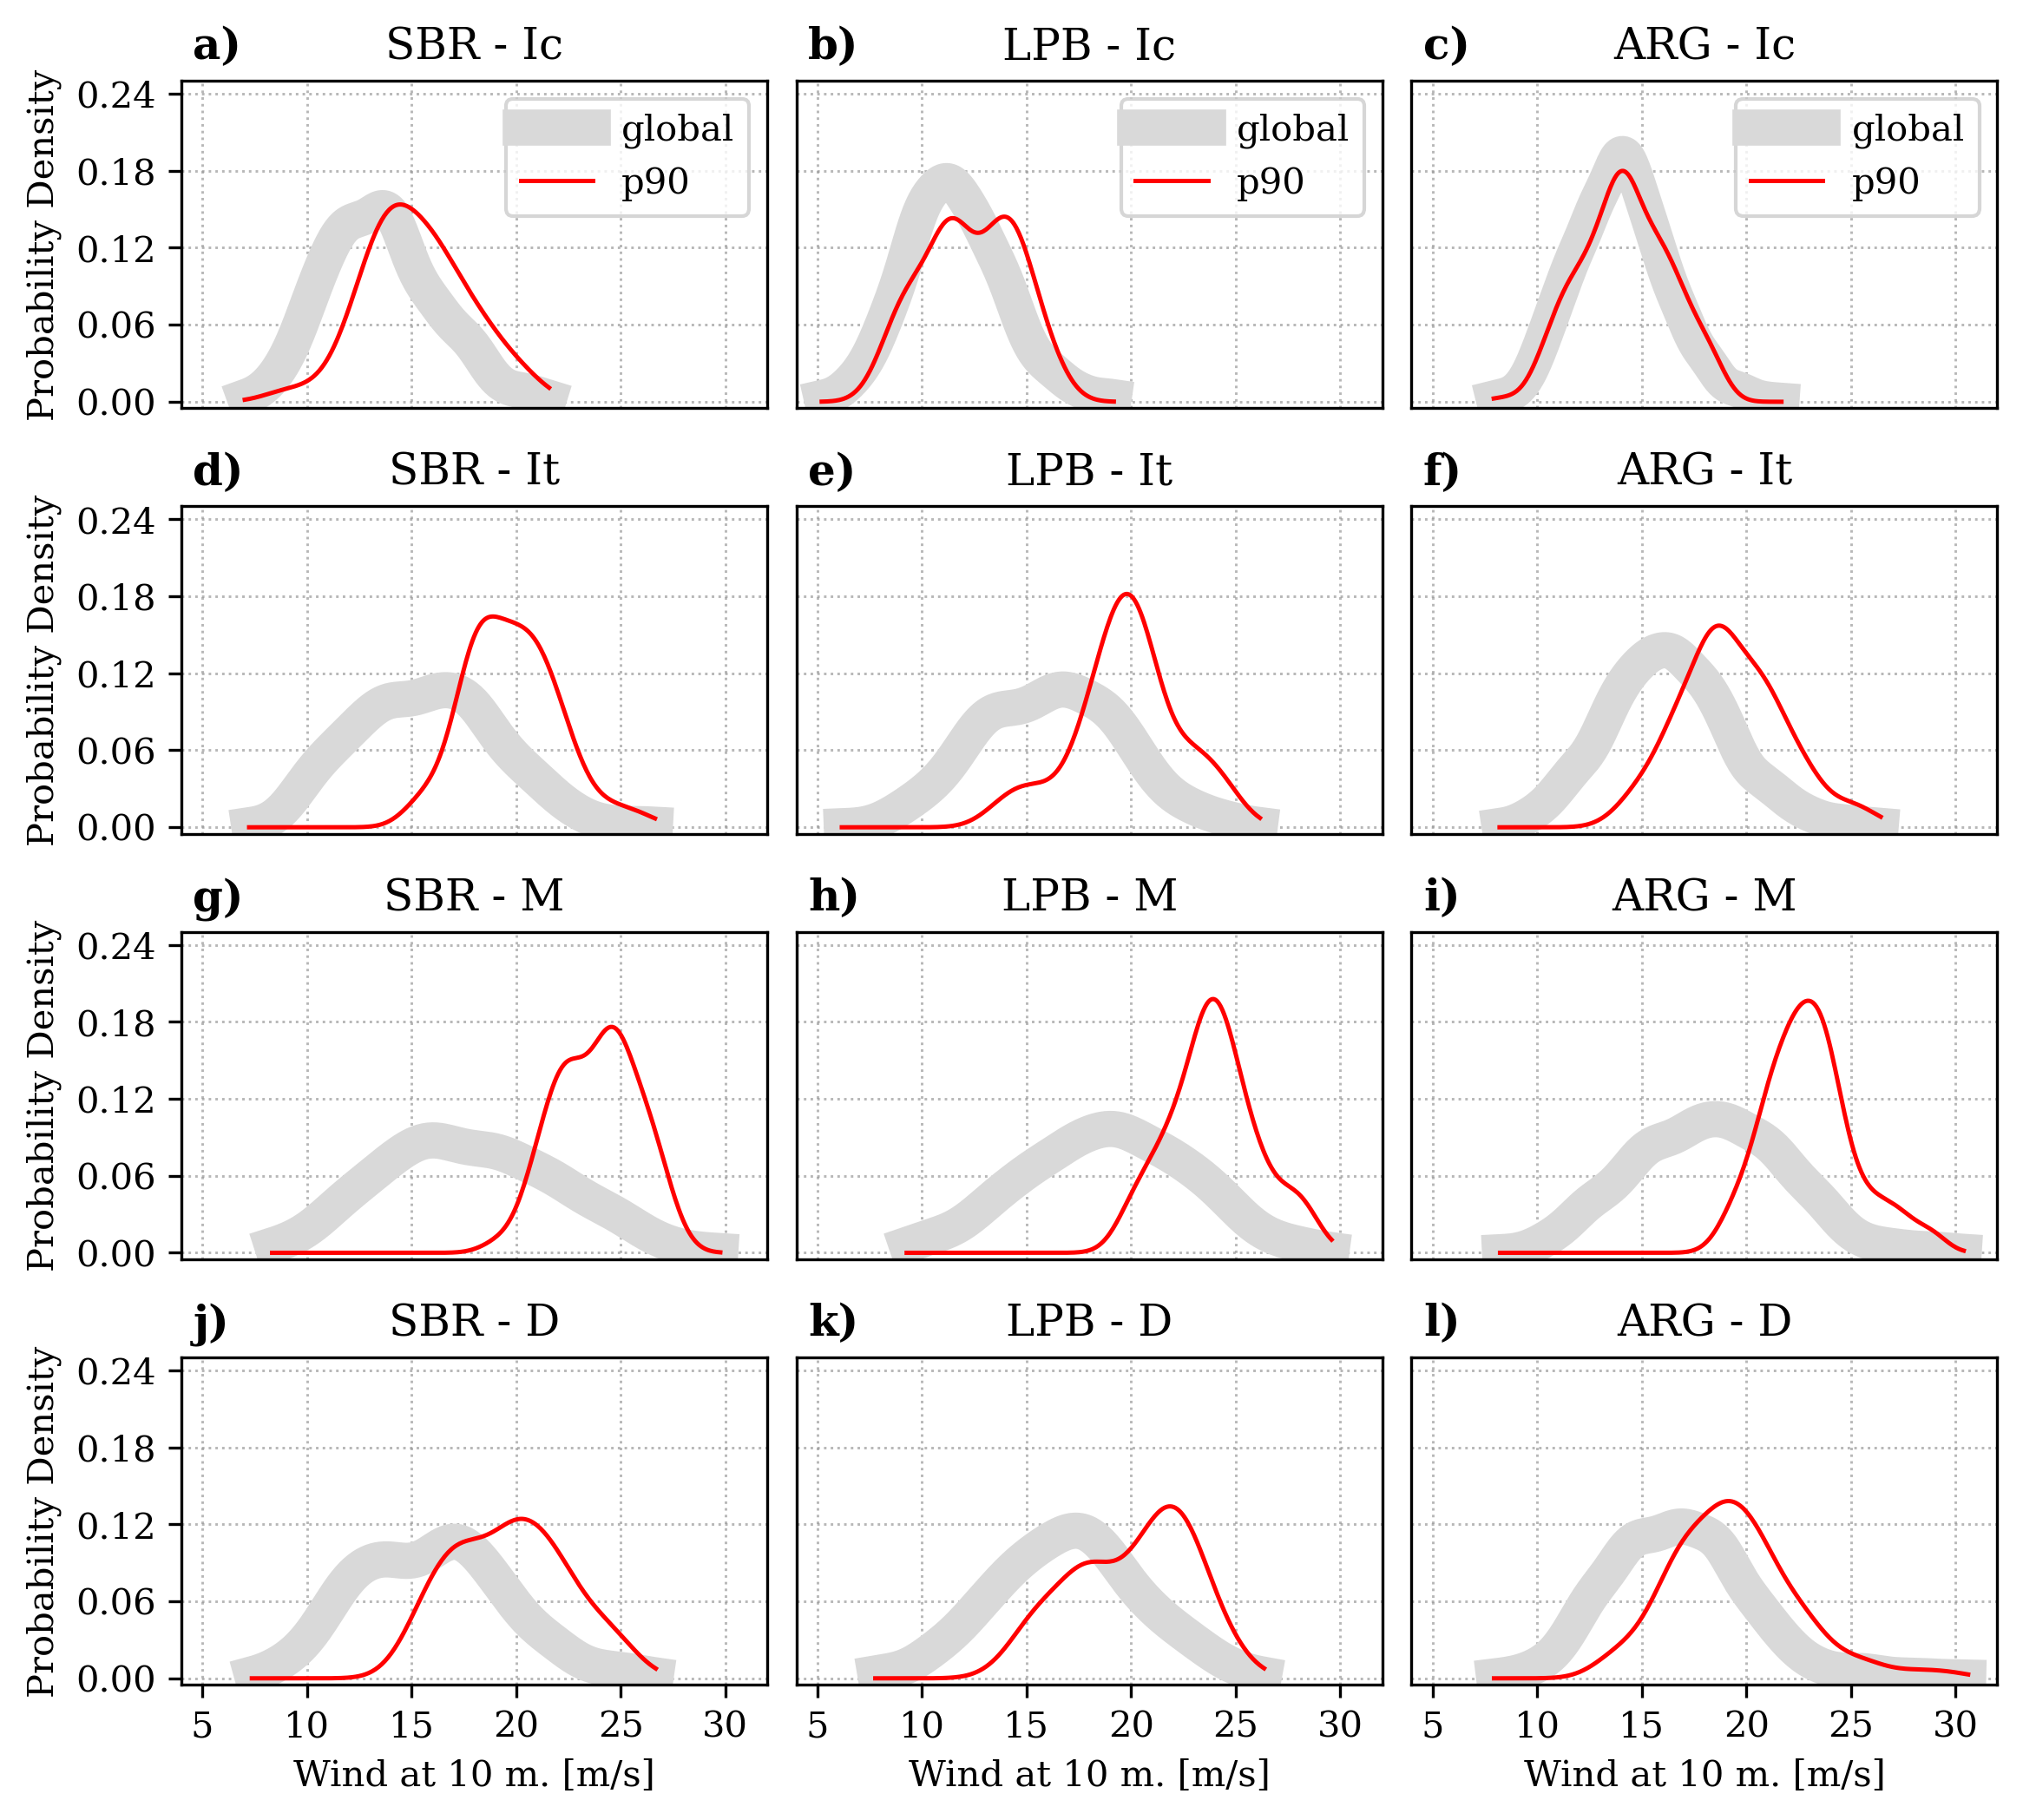
\includegraphics[width=\textwidth]{images/w10/PDF_wind10_sigma025.png}
\caption[PDF de magnitudes máximas de viento a 10 metros]{Funciones de densidad de probabilidad (PDF) para las magnitudes máximas de viento a 10 metros. Las columnas indican la región de ciclogénesis (SBR, LPB, ARG) y las filas la evolución a través de las fases del ciclo de vida (Ic, It, M, D). Se contrasta la población global (referencia, sombreado gris) con los subconjuntos definidos por percentiles de los máximos de vorticidad relativa en 850 hPa alcanzados en su ciclo vital: p10 (sistemas débiles, azul punteado), p50 (sistemas moderados, verde continuo) y p90 (sistemas extremos, rojo seccionado).}
\label{fig:pdf_wind10}
\end{figure}

La Figura \ref{fig:pdf_wind10} presenta un conjunto de funciones de densidad de probabilidad las cuales describen la distribución estadística de los máximos del viento en superficie a 10 metros. Estos valores máximos fueron extraídos del dominio lagrangiano de $20^\circ \times 20^\circ$ centrado en el núcleo de cada sistema. Esta dimensión espacial es consistente con enfoques metodológicos previos aplicados en el Atlántico Sudoccidental, como el de \citet{cardoso2022synoptic}, diseñados específicamente para capturar los vientos extremos que pueden ocurrir a varios cientos de kilómetros del centro del ciclón. La muestra global se encuentra estratificada por región de ciclogénesis (SBR, LPB, ARG) y dividida en subconjuntos de intensidad dinámica definidos según el pico máximo absoluto de vorticidad alcanzado durante todo el ciclo de vida de cada ciclón: sistemas débiles (p10), sistemas moderados (p50) y eventos extremos (p90). Transversalmente, la evolución de estos grupos estáticos se evalúa a lo largo de las cuatro fases de desarrollo (Ic, It, M, D).
% CITA TEXTUAL CARDOSO (2022): [Pega aquí la frase exacta de Cardoso sobre la justificación del radio de captura o el uso de dominios amplios para evaluar la estructura de los ciclones en nuestra región]

Durante la fase incipiente (Ic; paneles a, b y c), las distribuciones para todos los estratos de intensidad presentan una morfología unimodal estrecha y parcialmente superpuesta, con frecuencias máximas concentradas en el rango de 10 a 17 m/s. A medida que los sistemas evolucionan independientemente hacia las fases de intensificación (It; paneles d, e y f) y madurez (M; paneles g, h e i), se hace evidente la divergencia entre los grupos: la curva del subconjunto extremo (p90) se desplaza drásticamente hacia la derecha, alcanzando en la fase M un pico modal en el rango de 20 a 22 m/s y colas extendi\'endose hasta los 30 m/s. Este comportamiento lo distancia claramente de la curva moderada (p50), que mantiene su máximo alrededor de los 15 a 17 m/s, solapándose frecuentemente con la población de referencia. Regionalmente, en la etapa de madurez de SBR (g), el p90 exhibe un pico de densidad
agudo ($\sim$0.18) y acotado en altas velocidades; LPB (h) presenta igualmente un desplazamiento hacia velocidades mayores, aunque con un pico m\'as bajo y distribuci\'on m\'as extendida ($\sim$0.07), mientras que ARG (i) muestra la distribuci\'on p90 m\'as ancha y aplanada de las tres regiones, evidenciando una mayor heterogeneidad en la intensidad de sus sistemas extremos. Finalmente, en la fase de decaimiento (D; paneles j, k y l), las curvas p90 retroceden levemente hacia magnitudes menores y aumentan su dispersión, preservando no obstante una separación inconfundible respecto a los sistemas más débiles.

La máxima separación de las distribuciones en la fase de madurez refleja el momento en que los ciclones expresan su pleno potencial dinámico, alcanzando su mínimo absoluto de vorticidad relativa a 850 hPa y maximizando el gradiente horizontal de presión superficial. La marcada diferencia del subconjunto p90 evidencia que estos vórtices poseen, desde su génesis, un entorno o forzante más inestable que culmina en campos de viento sustancialmente más severos que un desarrollo estándar. 
%%
Las variaciones interregionales reflejan distintos forzamientos físicos predominantes. Tal como sostiene \citet{gramcianinov2024early}, los sistemas en las regiones SBR y LPB alcanzan intensidades de viento más extremas debido a la fuerte influencia de procesos termodinámicos en niveles bajos —como la advección cálida y la convergencia de humedad de origen oceánico y continental—, factores que los modelos de alta resolución logran representar con mayor fidelidad. Esta dependencia termodinámica se ilustra en el análisis del ciclón Raoni realizado por \citet{reboita2022from}, donde se evidenció que los flujos turbulentos de calor sensible y latente desde el océano, junto con el transporte de humedad continental por vientos, fueron decisivos para fortalecer el sistema y organizar la convección. Asimismo, experimentos numéricos confirman que la representación precisa de estos intercambios de calor en superficie es esencial para capturar la intensificación de los vientos en niveles bajos. Este aspecto termodinámico es estudiado por \citet{russo2025impacts}, quienes demuestran que la inyección masiva de humedad y flujos de calor latente concentra la energía cinética y favorece el desarrollo baroclínico de sistemas severos.
% REFERENCIA TEXTUAL 
% "gramcianinov2024early The GCMs tend to underestimate the wind intensity in all regions... The RCMs are generally closer to the ERA5 wind speed distribution but with an overestimation of the cyclones' winds, as depicted by the high probability in the right-hand tail".
% RUSSO ET AL. (2025): "The results indicate that latent heat flux associated with SST plays a fundamental role in baroclinic development... Specific humidity in the warm sector was a crucial factor in the intensification of all the cases studied."
Mientras tanto, en ARG, la dinámica baroclínica clásica del frente polar y la perturbación topográfica de los Andes generan respuestas cinemáticas más variables y distribuciones más aplanadas. De acuerdo con \citet{gan1994influence}, la cordillera induce severas distorsiones espaciales en el flujo de niveles bajos, mientras que \citet{vera2002cold} detallan la profunda modificación en la estructura tridimensional de las ondas al cruzar el relieve andino. Esta modulación orográfica explica la mayor heterogeneidad e irregularidad geométrica en el campo de vientos superficiales para los sistemas generados en esta región.
% REFERENCIA TEXTUAL GAN Y RAO (1994): "When the wave approaches the Andes Cordillera, it exhibits orographic effects such as anticyclonic turning of a low-level disturbance trajectory, a zonal trajectory in the upper levels, distortions of the isolines of correlation, and an elongation of maximum correlation on the lee side of the Andes."
% REFERENCIA TEXTUAL VERA ET AL. (2002): "Both cyclonic and anticyclonic perturbations display significant modifications in their three-dimensional structure as they evolve over extratropical and subtropical South America."
La cuantificación de estas distribuciones permite comparar objetivamente cómo evolucionan las magnitudes más probables y la extensión de los valores extremos entre ciclones de distinta génesis. Al confirmar que los ciclones clasificados dinámicamente como extremos (p90) se separan sistemáticamente de la población a medida que maduran, se valida la pertinencia de la clasificación basada en vorticidad. En la fase de madurez, mientras que la moda de los sistemas débiles (p10) se sitúa en torno a los 12-15 m/s, el grupo p90 desplaza su mayor probabilidad hacia los 22 m/s, lo que representa un incremento de aproximadamente el 50\% en la intensidad del viento más frecuente. Las colas en las distribuciones p90 alcanzan magnitudes críticas de hasta 30 m/s. Este corrimiento coincide con los registros documentados por \citet{padilhareinke2026characterization} y \citet{gramcianinov2020analysis} para los eventos severos del Atlántico Sur. \citet{padilhareinke2026characterization} reportan una intensidad media de viento a 10 metros de 70.0 km/h ($\approx$ 19.4 m/s), con un umbral para eventos intensos (p90) de 84.4 km/h ($\approx$ 23.4 m/s) y magnitudes extremas que alcanzan hasta 113.21 km/h ($\approx$ 31.4 m/s) en las colas de la distribución. Estos rangos son consistentes con lo documentado por \citet{gramcianinov2020analysis}, quienes reportan, para el invierno austral (JJA), velocidades máximas medias de entre 21.2 ± 4.8 m/s y 23.4 ± 4.8 m/s, con valores del percentil 90 de entre 27.3 y 30.2 m/s y del percentil 95 de hasta 32.1 m/s en bases de datos de alta resolución como CFSR/CFSv2. Desde una perspectiva analítica, lo observado en el Hemisferio Norte por \citet{corner2025classification}, quienes emplean un método de clasificación de ciclones distinto, se identifica que el grupo de los ciclones más débiles presenta una moda en la velocidad del viento a 10 metros de 12.5 m/s. En contraste, ciclones más intensos alcanzan los 22.5 m/s. Las colas en las distribuciones de este grupo extremo alcanzan magnitudes críticas de hasta 35 m/s, lo que confirma que estos sistemas mantienen consistentemente sus valores de viento por encima del umbral de los 20 m/s.
%
Como subraya \citet{gramcianinov2023impact}, identificar tempranamente sistemas extremos resulta indispensable, ya que estos vientos anómalos son los forzantes primarios en la generación de oleaje destructivo y suponen un riesgo directo para las regiones costeras y marítimas.
% CITA TEXTUAL GRAMCIANINOV (2023): "Explosive cyclones over the South Atlantic show highly localized extreme wind cores, which are the primary drivers for the generation of severe wave events."

% ==============================================================================
% SECCIÓN PRINCIPAL: KDE ESPACIAL DE VIENTO A 10 METROS
% ==============================================================================
%
\section{Distribución espacial de máximos (KDE)}
% $$$$
\subsection{Población Global}\label{sec:kde_espacial_global}

\begin{figure}[htbp]
\centering
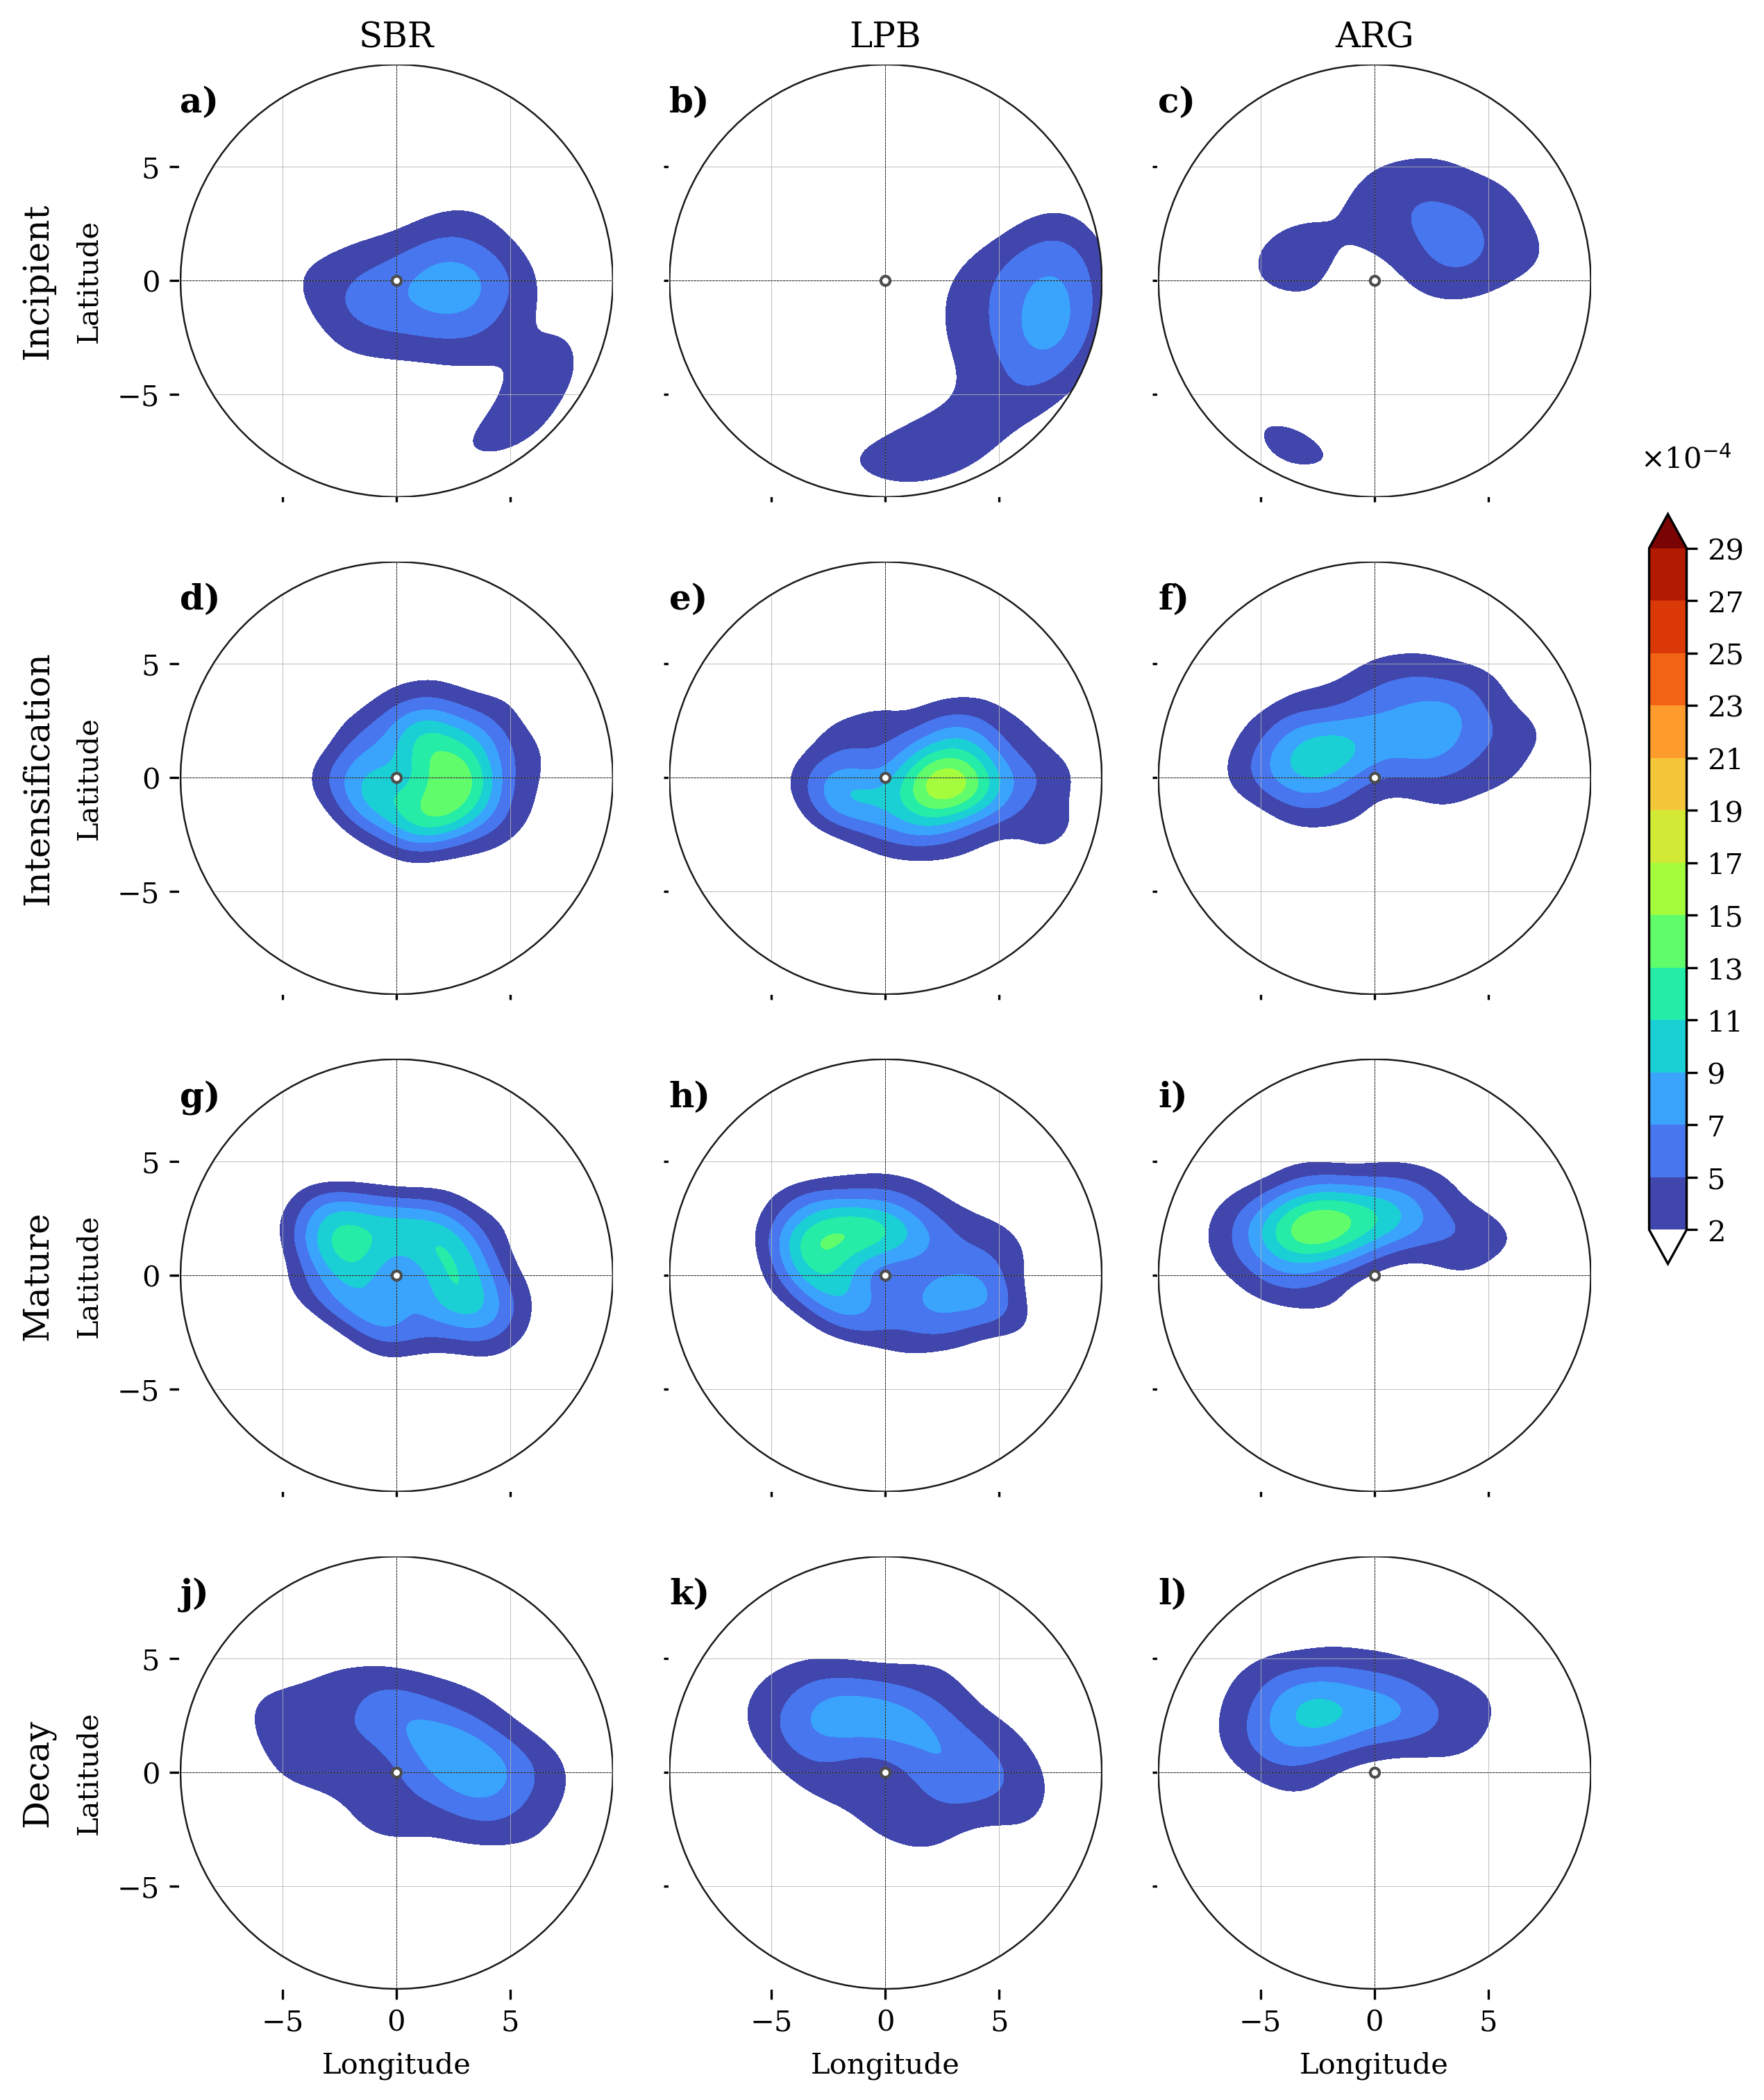
\includegraphics[width=\textwidth]{images/w10/kde_wind10_global_fasesxreg.png}
\caption[PDF espacial de viento máximo a 10 metros - Población Global]{Estimación de densidad espacial bidimensional de la ubicación de los máximos de magnitud de viento a 10 metros para la Población Global. Las columnas separan las regiones de ciclogénesis (SBR, LPB, ARG) y las filas indican las fases evolutivas (Ic, It, M, D). El dominio lagrangiano está centrado en el ciclón ($0^\circ, 0^\circ$).}
\label{fig:kde_wind_global}
\end{figure}

La Figura~\ref{fig:kde_wind_global} presenta el campo de densidad espacial sobre el dominio lagrangiano de $20^\circ \times 20^\circ$ previamente definido. A nivel global, la distribución se caracteriza por ser amplia, difusa y con gradientes de probabilidad suaves. En las fases iniciales (Ic; paneles a, b y c), las zonas de máxima densidad abarcan áreas extensas que no definen una estructura simétrica alrededor del centro del ciclón. Esta falta de organización inicial concuerda con lo expuesto por \citet{reboita2010south} y \citet{gozzo2017climatology}, quienes señalan la alta variabilidad de los sistemas que componen la población general, incluyendo una abundante ocurrencia de ciclones débiles o someros cuya circulación no logra consolidar un patrón simétrico de vientos en sus primeras etapas.
% CITA TEXTUAL Gozzo et al. (2014/2017): "the abundant occurrence of shallow cyclonic systems, especially near the southeastern Brazilian coast, that do not reach sustained winds of 17 m s-1 but may cause notable weather events"
% CITA TEXTUAL Reboita et al. (2010): "Considering the systems initiate with [weaker vorticity -1.5 x 10(-5) s(-1)], the annual cycle is not well defined... The stronger systems [...] have a well-characterized high frequency"
A medida que los sistemas avanzan hacia la madurez (M; paneles g, h e i), se observa una leve preferencia de localización en el cuadrante noroeste, manteniendo diferencias posicionales entre regiones. Como sugiere \citet{dossantos2023response}, esta evolución espacial asimétrica está ligada a las zonas baroclínicas, donde los máximos gradientes térmicos horizontales interactúan con los chorros en la alta troposfera.
% CITA TEXTUAL dos Santos et al. (2023): "This type of instability occurs at medium latitudes, in the so-called baroclinic zones, where the maximum horizontal temperature gradients are located on a large scale and where jets are consequently observed in the upper troposphere."
En esta etapa, la densidad m\'axima en ARG (i) alcanza valores de $\approx$\,19--21 $\times 10^{-4}$, mientras que SBR (g) y LPB (h) alcanzan mayor densidad en \'areas m\'as restringidas, indicando un foco más recurrente para la localización de vientos máximos. Este contraste regional responde a forzantes distintos: mientras que los sistemas en ARG están modulados principalmente por la advección térmica, la mayor concentración en SBR y LPB se favorece por la advección de aire cálido y húmedo junto al desarrollo de bajas orográficas en etapas iniciales \citep{gramcianinov2019properties, cardoso2022synoptic}.
% CITA TEXTUAL Gramcianinov et al. (2019): "The cyclone composites reveal that SE-BR [SBR] and SE-SAO cyclones are associated with secondary development, the LA PLATA [LPB] cyclones development is influenced by an orographic low in their early stages, and ARG cyclones are influenced by thermal advection as an essential mechanism in the reduction of static stability."
% CITA TEXTUAL Gramcianinov et al. (2019): "The increase in genesis at 30S over the continent is associated with the strengthening of the upper-level jet and the increase of warm and moisture advections at the same location."

Esta alta dispersión espacial es inherente al uso de un catálogo masivo donde los sistemas varían desde configuraciones débiles hasta atípicas. Como señala \citet{sinclair1994objective}, los métodos de identificación basados en vorticidad capturan un espectro amplio que incluye numerosos ciclones débiles, móviles y de menor duración. Físicamente, cuando la interacción baroclínica es débil, el flujo sinóptico de niveles medios o altos domina la circulación y el sistema es gobernado por anomalías en la alta troposfera que no logran consolidar un acoplamiento profundo, modificando la ubicación del viento máximo en función de gradientes de presión transitorios \citep{hoskins2005new}.
% CITA TEXTUAL Sinclair (1994): "The vorticity-based climatology includes many more weak, mobile, and short-lived weather systems than are found from MSLP analyses."
% CITA TEXTUAL Hoskins y Hodges (2005): "In the absence of strong baroclinic development, upper-tropospheric features can exist and propagate without a significant low-level signature [...] leading to a weaker coupling."
La caracterización de esta dispersión establece la línea base climatológica esencial: demuestra que, en la población general, el máximo de viento puede ocurrir en un radio muy amplio y variable. Esta heterogeneidad justifica metodológicamente la estratificación por intensidad, respaldada por \citet{corner2025classification} y \citet{eisenstein2023identification}, quienes destacan que la diversidad de estos sistemas exige clasificarlos para aislar los eventos severos. Aunque esta estratificación es habitual en el Hemisferio Norte, su aplicación sistemática en el Hemisferio Sur permanece como necesidad crítica. El contraste contra esta línea 
base revela inmediatamente la organización geométrica de los sistemas extremos, cuya arquitectura espacial se examina a continuación.
% CITA TEXTUAL Corner et al. (2025): "Given the large number and variety of extratropical cyclones, objective classification is necessary to understand their diverse physical characteristics and impacts."
% CITA TEXTUAL Eisenstein et al. (2023): "To fully understand the spectrum of cyclone impacts, it is essential to distinguish between the large number of weak systems and the minority of intense storms that produce severe weather."

\subsection{Subconjunto extremo (p90)}\label{sec:kde_espacial_p90}

\begin{figure}[htbp]
\centering
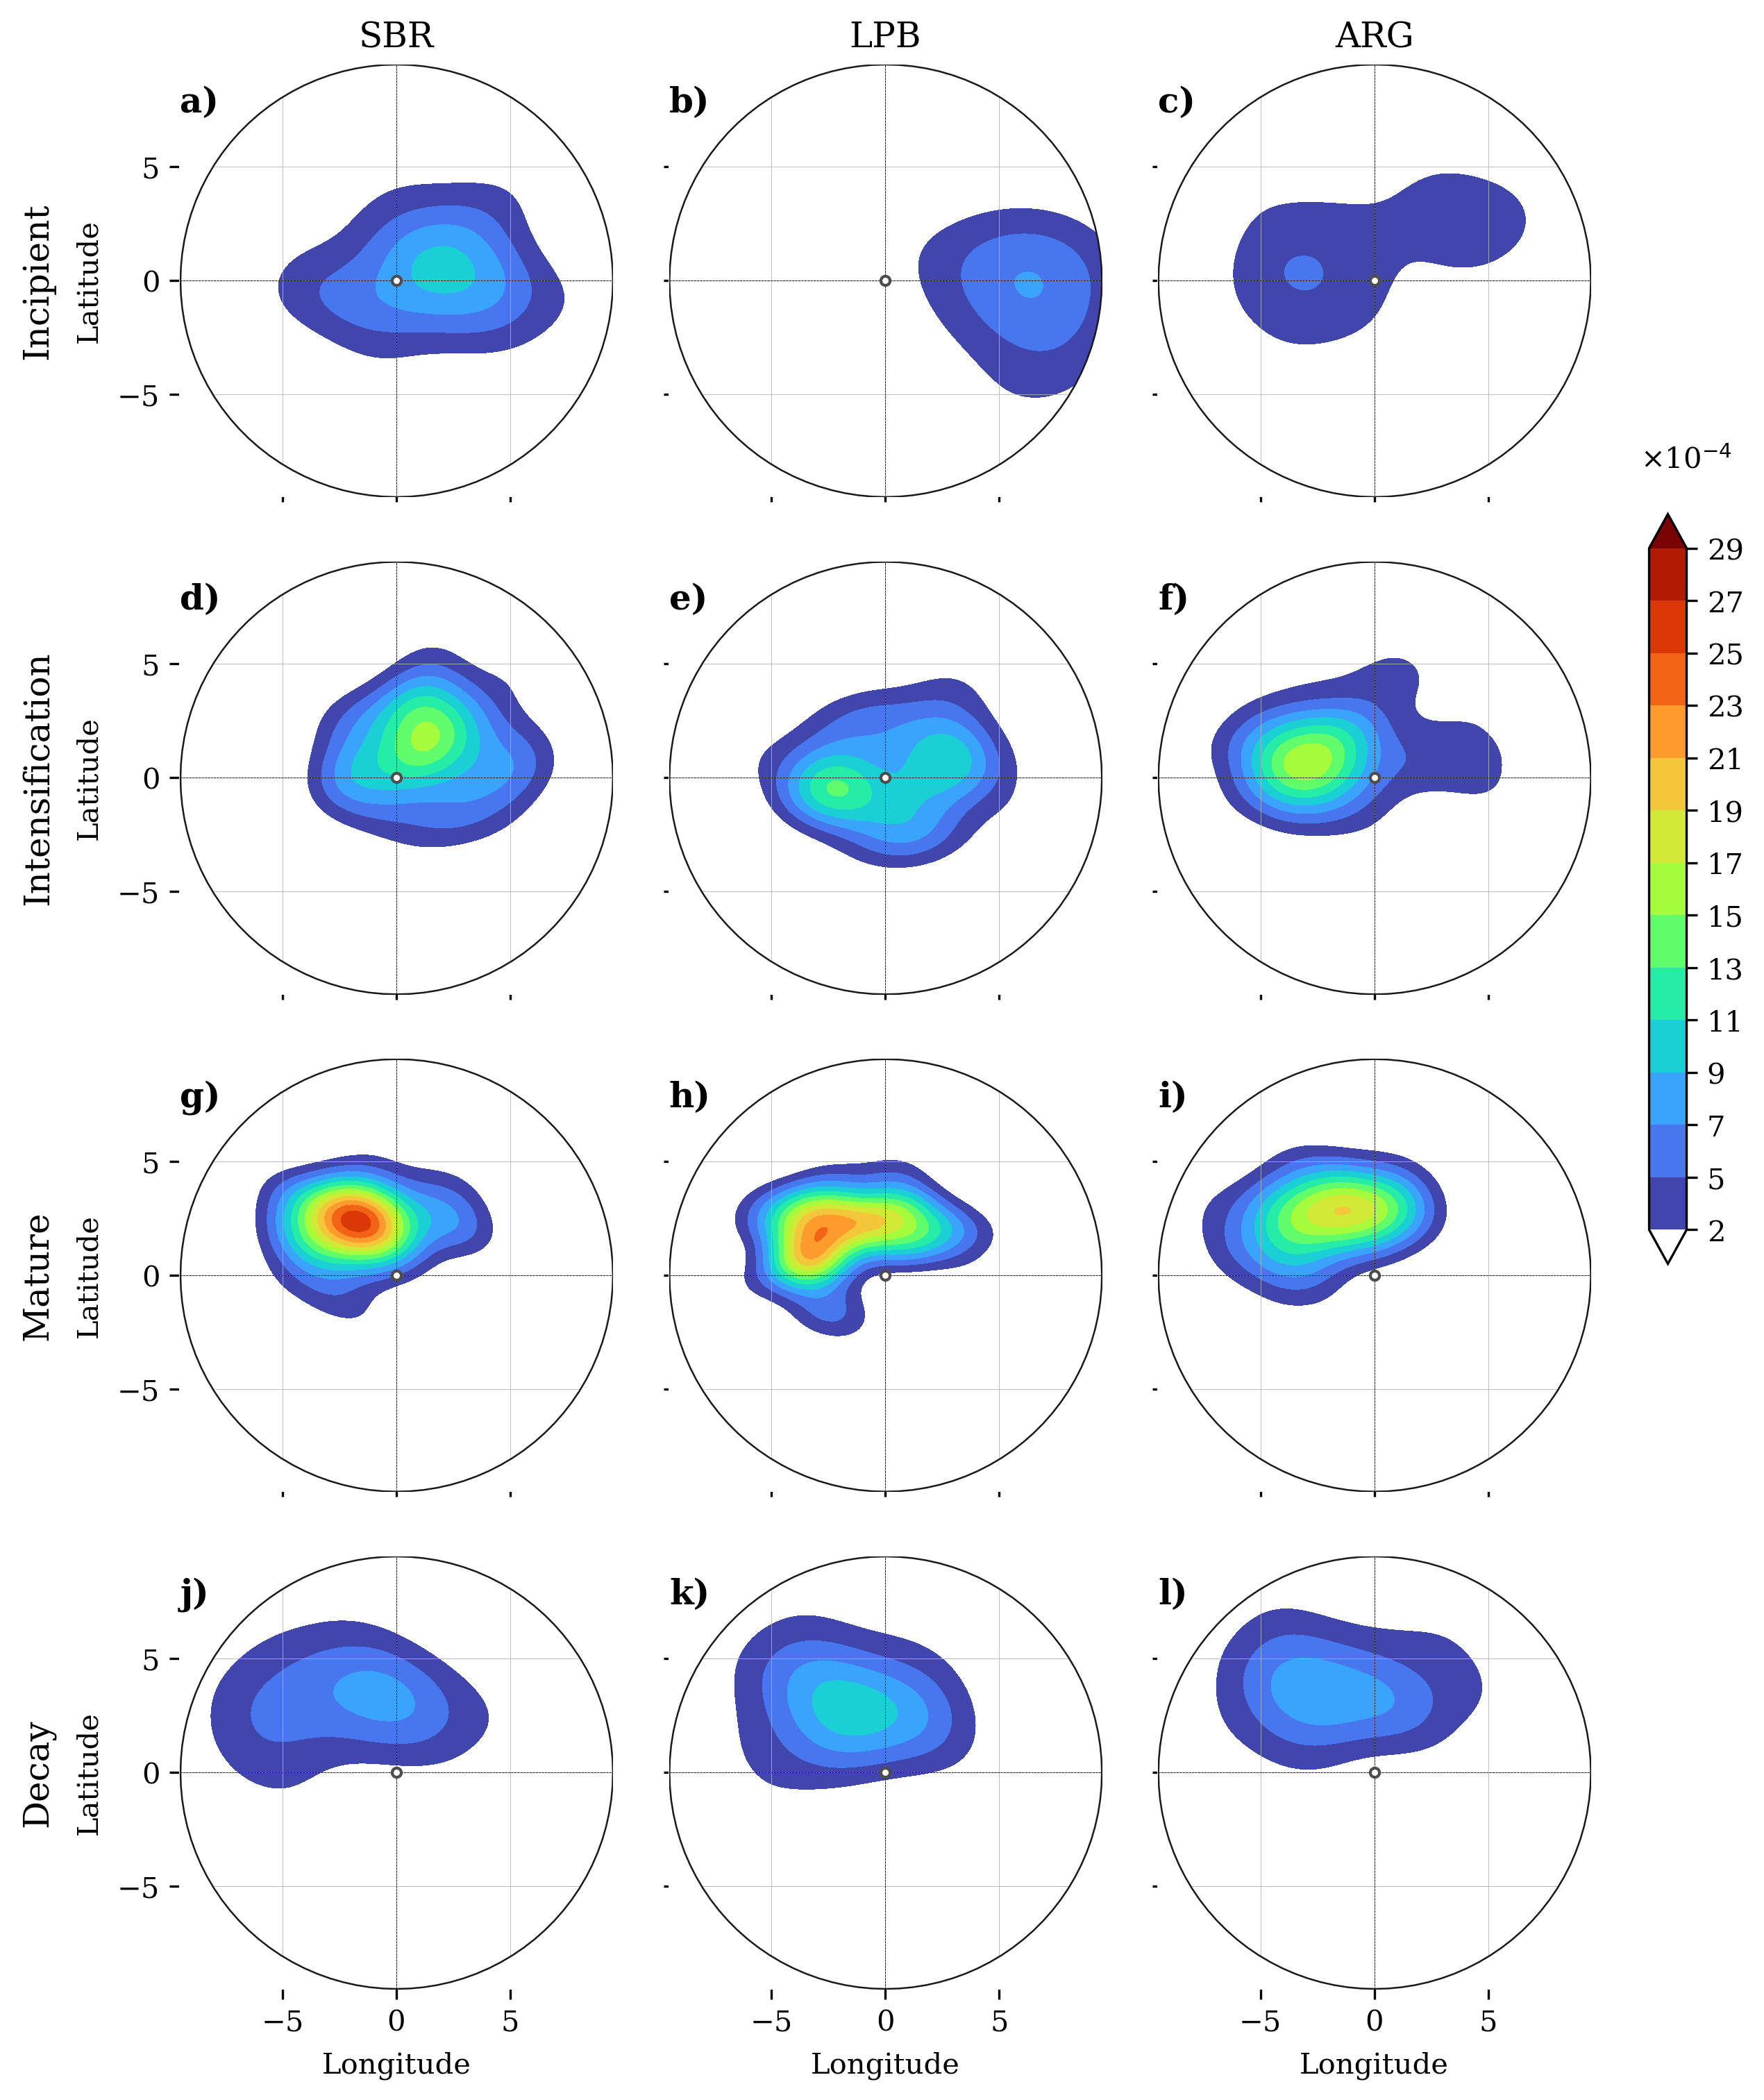
\includegraphics[width=\textwidth]{images/w10/kde_wind10_p90_fasesxreg.png}
\caption[PDF espacial de viento máximo a 10 metros - Subconjunto p90]{Estimación de densidad espacial bidimensional de la ubicación de los máximos de magnitud de viento a 10 metros para el subconjunto de ciclones intensos. El formato, dominio lagrangiano, fases evolutivas y escala de densidad ($10^{-4}$) son idénticos a los presentados en la Figura~\ref{fig:kde_wind_global} para permitir la comparación estructural directa de las asimetrías de densidad.\footnote{Los mapas correspondientes a los estratos de menor intensidad (p10 y p50) se documentan en el Apéndice~\ref{apendice:kde_espacial} para referencia complementaria.}}
\label{fig:kde_wind_p90}
\end{figure}

Al contrastar esta línea base contra el estrato de sistemas extremos (p90), la reorganización espacial resulta drástica. La Figura~\ref{fig:kde_wind_p90} revela que la arquitectura de los vientos máximos deja de ser difusa para configurar un n\'ucleo de alta densidad marcadamente concentrado en el cuadrante noroeste durante la fase de madurez (M; paneles g, h e i), localizado aproximadamente a $-1^{\circ}$ a $-2^{\circ}$ de longitud y entre $+1^{\circ}$ y $+2^{\circ}$ de latitud relativa al centro. Las magnitudes de densidad alcanzadas en SBR (g) son particularmente
extremas (valores entre 23 y $27 \times 10^{-4}$, tonos naranja--rojizos), mientras que LPB (h) alcanza valores de $\approx$\,23--25\,$\times 10^{-4}$, denotando una recurrencia espacial altísima para la localización de los vientos máximos. Por su parte, ARG (i) exhibe igualmente una concentración respecto a la población global, aunque con un núcleo de densidad comparativamente menor y ligeramente más disperso que sus contrapartes oceánicas. En la fase de decaimiento (D; paneles j, k y l), este núcleo asimétrico se mantiene anclado en el sector noroeste, a diferencia del comportamiento errático observado en la población general durante esta etapa.

Esta hiperconcentración en el cuadrante noroeste (Hemisferio Sur) constituye la firma espacial de los ciclones profundos maduros. Como ha sido documentado para el Hemisferio Norte (cuadrante suroeste) por \citet{clark2005sting} y \citet{han2025system}, los sistemas extratropicales más intensos empaquetan sus vientos extremos en el sector posterior, asociados específicamente a la zona de fractura frontal y al desarrollo de intensas corrientes en chorro de niveles bajos (\textit{sting jet} o cinta transportadora fría). Al aplicar el efecto espejo producto de la circulación ciclónica inversa entre hemisferios, la configuración dinámica del sector posterior correspondería espacialmente al cuadrante noroeste. Físicamente, la consolidación de este núcleo extremo responde a procesos de transferencia de cantidad de movimiento: en las inmediaciones del frente frío se desarrollan intensas corrientes descendentes que transportan el momento horizontal de la alta troposfera hacia la capa límite \citep{hyeok2024extrem}. No obstante, debe considerarse que los datos de reanálisis ERA5 pueden subestimar la intensidad real del viento debido a limitaciones de resolución. Como demuestran \citet{gentile2023}, los chorros de la cinta transportadora fría (CCBb) en ciclones maduros están asociados con capas límite significativamente más profundas, potenciadas por la inestabilidad que genera el aire frío al circular sobre aguas oceánicas relativamente cálidas; esto induce flujos de calor positivos que facilitan una mezcla vertical descendente altamente eficiente de aire de alta velocidad hacia la superficie, manifestándose en el KDE como un empaquetamiento localizado a 10 metros, sector donde el CCBb constituye el principal motor de riesgos de viento a pesar de que modelos como ERA5 tienden a subestimar estas intensidades en aproximadamente 4.5~m~s$^{-1}$.
% CITA TEXTUAL Clark et al. (2005): "The sting jet is a transient mesoscale airflow that descends from the cloud head into the frontal-fracture region, producing damaging surface winds."
% CITA TEXTUAL Han et al. (2025): "For the most intense extratropical cyclones, extreme winds are predominantly associated with the cold conveyor belt and sting jets, concentrating in the rear-left [northwest] quadrant relative to the storm center."
% CITA TEXTUAL Reboita et al. (2018): "Cyclones developing over the western South Atlantic are strongly influenced by the Brazil Current, where sensible and latent heat fluxes contribute significantly to rapid intensification."
% CITA TEXTUAL Gramcianinov et al. (2023): "Explosive cyclones over the South Atlantic show highly localized extreme wind cores, which are the primary drivers for the generation of severe wave events."

Las diferencias interregionales observadas en la Figura~\ref{fig:kde_wind_p90} —particularmente la mayor concentración en SBR y LPB respecto a ARG— respaldan este marco dinámico. Por un lado, \citet{reboita2018extratropical} destaca que el Atlántico Sudoccidental es un entorno donde las interacciones diabáticas y los fuertes flujos de calor latente océano-atmósfera fomentan la rápida intensificación de los sistemas. Conectando estos procesos térmicos con una zonificación específica, \citet{gramcianinov2023impact} señala que los ciclones originados particularmente en SBR y LPB capitalizan estas condiciones para generar desarrollos de tipo explosivo, empaquetando el momento cinético en un sector espacial muy estrecho. Por el contrario, en ARG, la dinámica baroclínica clásica del frente polar y la perturbación topográfica de los Andes generan estructuras marginalmente más elongadas que dejarán las ubicaciones de los máximos de viento menos concentradas.

La cuantificación de esta concentración demuestra que el grado de severidad de un ciclón predetermina su patrón espacial. Los sistemas extremos originados en el Atlántico Sur concentrarán casi invariablemente sus máximos de viento a 10 metros en un radio y cuadrante particular respecto a su centro. Tal como destaca \citet{dalanhese2023new} para el litoral sudamericano, esta previsibilidad geométrica es una herramienta importante para conocer la espacialidad de las posibles afectaciones que puedan ocurrir durante estos eventos severos.

% CITA TEXTUAL Dalanhese et al. (2023): "Accurate forecasting of the spatial distribution of extreme winds is critical to improve early warning systems and mitigate structural damage to coastal regions in southern Brazil."


% ==============================================================================
% SECCIÓN: PATRONES DOMINANTES DE VARIABILIDAD (EOF) - VIENTO A 10 METROS
% ==============================================================================
\section{Organización estructural: Análisis EOF}\label{sec:eof_wind10}
\subsection{Fraccionamiento de varianza}\label{sec:var_exp_wind10}

\begin{figure}[!ht]
\centering
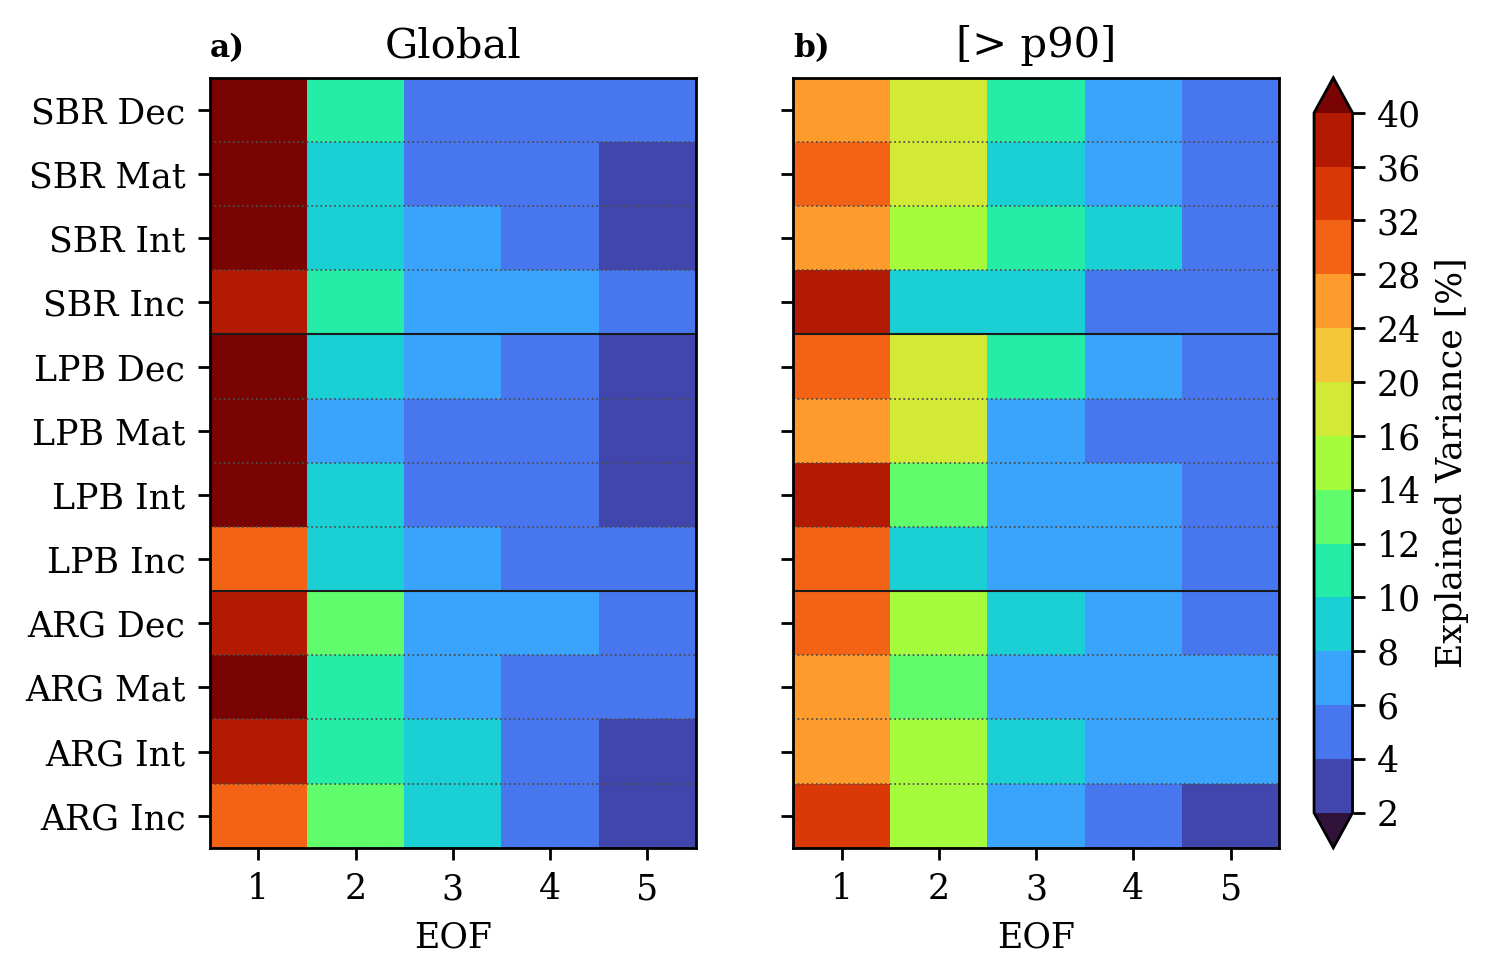
\includegraphics[width=\textwidth]{images/w10/all_expvar_wind10_mean2times.png} 
\caption[Varianza explicada por los primeros cinco modos (EOF1-EOF5) de viento a 10 m]{Fraccionamiento de la varianza espacial total contenida en los primeros cinco modos dominantes (EOF1 a EOF5) del viento a 10 metros. Se contrasta la distribución de la varianza de la Población Global frente a los estratos de intensidad (p10, p50 y p90) a lo largo del ciclo de vida para cada región de ciclogénesis.}
\label{fig:var_exp_wind10}
\end{figure}

% ¿Qué es?
La Figura \ref{fig:var_exp_wind10} sintetiza el fraccionamiento de la varianza espacial distribuida en los primeros cinco modos ortogonales (EOF1 a EOF5) del campo de viento superficial. Este desglose permite evaluar la dimensionalidad y cohesión de la energía cinética. Se contrasta el comportamiento de la Población Global de referencia frente a los estratos de distinta intensidad dinámica intrínseca (p10, p50 y p90) a lo largo de las fases evolutivas.

% ¿Cómo es?
El análisis revela una divergencia drástica en la distribución de la varianza entre las poblaciones. En la Población Global, así como en los estratos de menor y media intensidad (p10 y p50), el modo EOF1 ejerce un dominio abrumador, capturando hasta el 57.1\% (LPB) y el 57.4\% (SBR) de la varianza durante la fase de madurez, que es donde el dominio del EOF1 resulta m\'as pronunciado en estas regiones. Esto genera una ca\'ida abrupta entre el primer modo y los modos de orden superior (EOF2 a EOF5), los cuales retienen porciones marginales de energía, confirmando que la dinámica de los sistemas p10 y p50 no altera la dimensionalidad base del sistema. Por el contrario, al evaluar el estrato extremo (p90), la concentración de varianza en EOF1 se reduce drásticamente: el EOF1 no logra superar el 37.6\% de representatividad, registrando mínimos de hasta 25.4\% durante la intensificación en ARG. Consecuentemente, la varianza del p90 se reparte y aplana, inflando la importancia relativa de los modos secundarios (EOF2 y EOF3).

% ¿Por qué es así?
La alta concentración de energía en un solo modo (EOF1) para el grupo global, p10 y p50 corrobora que en general los ciclones son gobernados por un gradiente de gran escala impuesto por el flujo sinóptico de fondo. Sin embargo, el aplanamiento de la varianza en los eventos severos (p90) confirma estadísticamente la fragmentación multiescalar. Tal como establece la teoría matemática de \citet{hannachi2007empirical}, un espectro de autovalores más plano es el indicador de que la energía de un sistema complejo se ha distribuido entre múltiples modos competitivos. Al intensificarse, el vórtice extremo genera perturbaciones internas no lineales: frentes excepcionalmente activos, corrientes en chorro de bajos niveles y seclusiones térmicas. Estas estructuras de mesoescala compiten entre sí por la energía cinética del campo, obligando a la descomposición matemática a utilizar múltiples dimensiones ortogonales (EOF2-EOF5) para poder reconstruir el caos cinemático del ciclón.

% ¿Para qué?
Esta métrica constituye una demostración cuantitativa irrefutable de que la severidad extrema no equivale a un simple escalado lineal de un ciclón ordinario. Concluir que los eventos extremos (p90) requieren múltiples dimensiones espaciales para ser explicados es crítico para la modelación numérica: demuestra que parametrizar vientos destructivos asumiendo los patrones simples de la población media subestimará sistemáticamente la agresividad, la naturaleza asimétrica y la localización real de las ráfagas.
% ==============================================================================
% ==============================================================================
\subsection{Patrones espaciales dominantes (EOF1)}\label{subsec:eof1_wind10}
% ==============================================================================
% ==============================================================================
\subsubsection{Población Global}\label{subsubsec:eof1_wind10_global}

\begin{figure}[htbp]
\centering
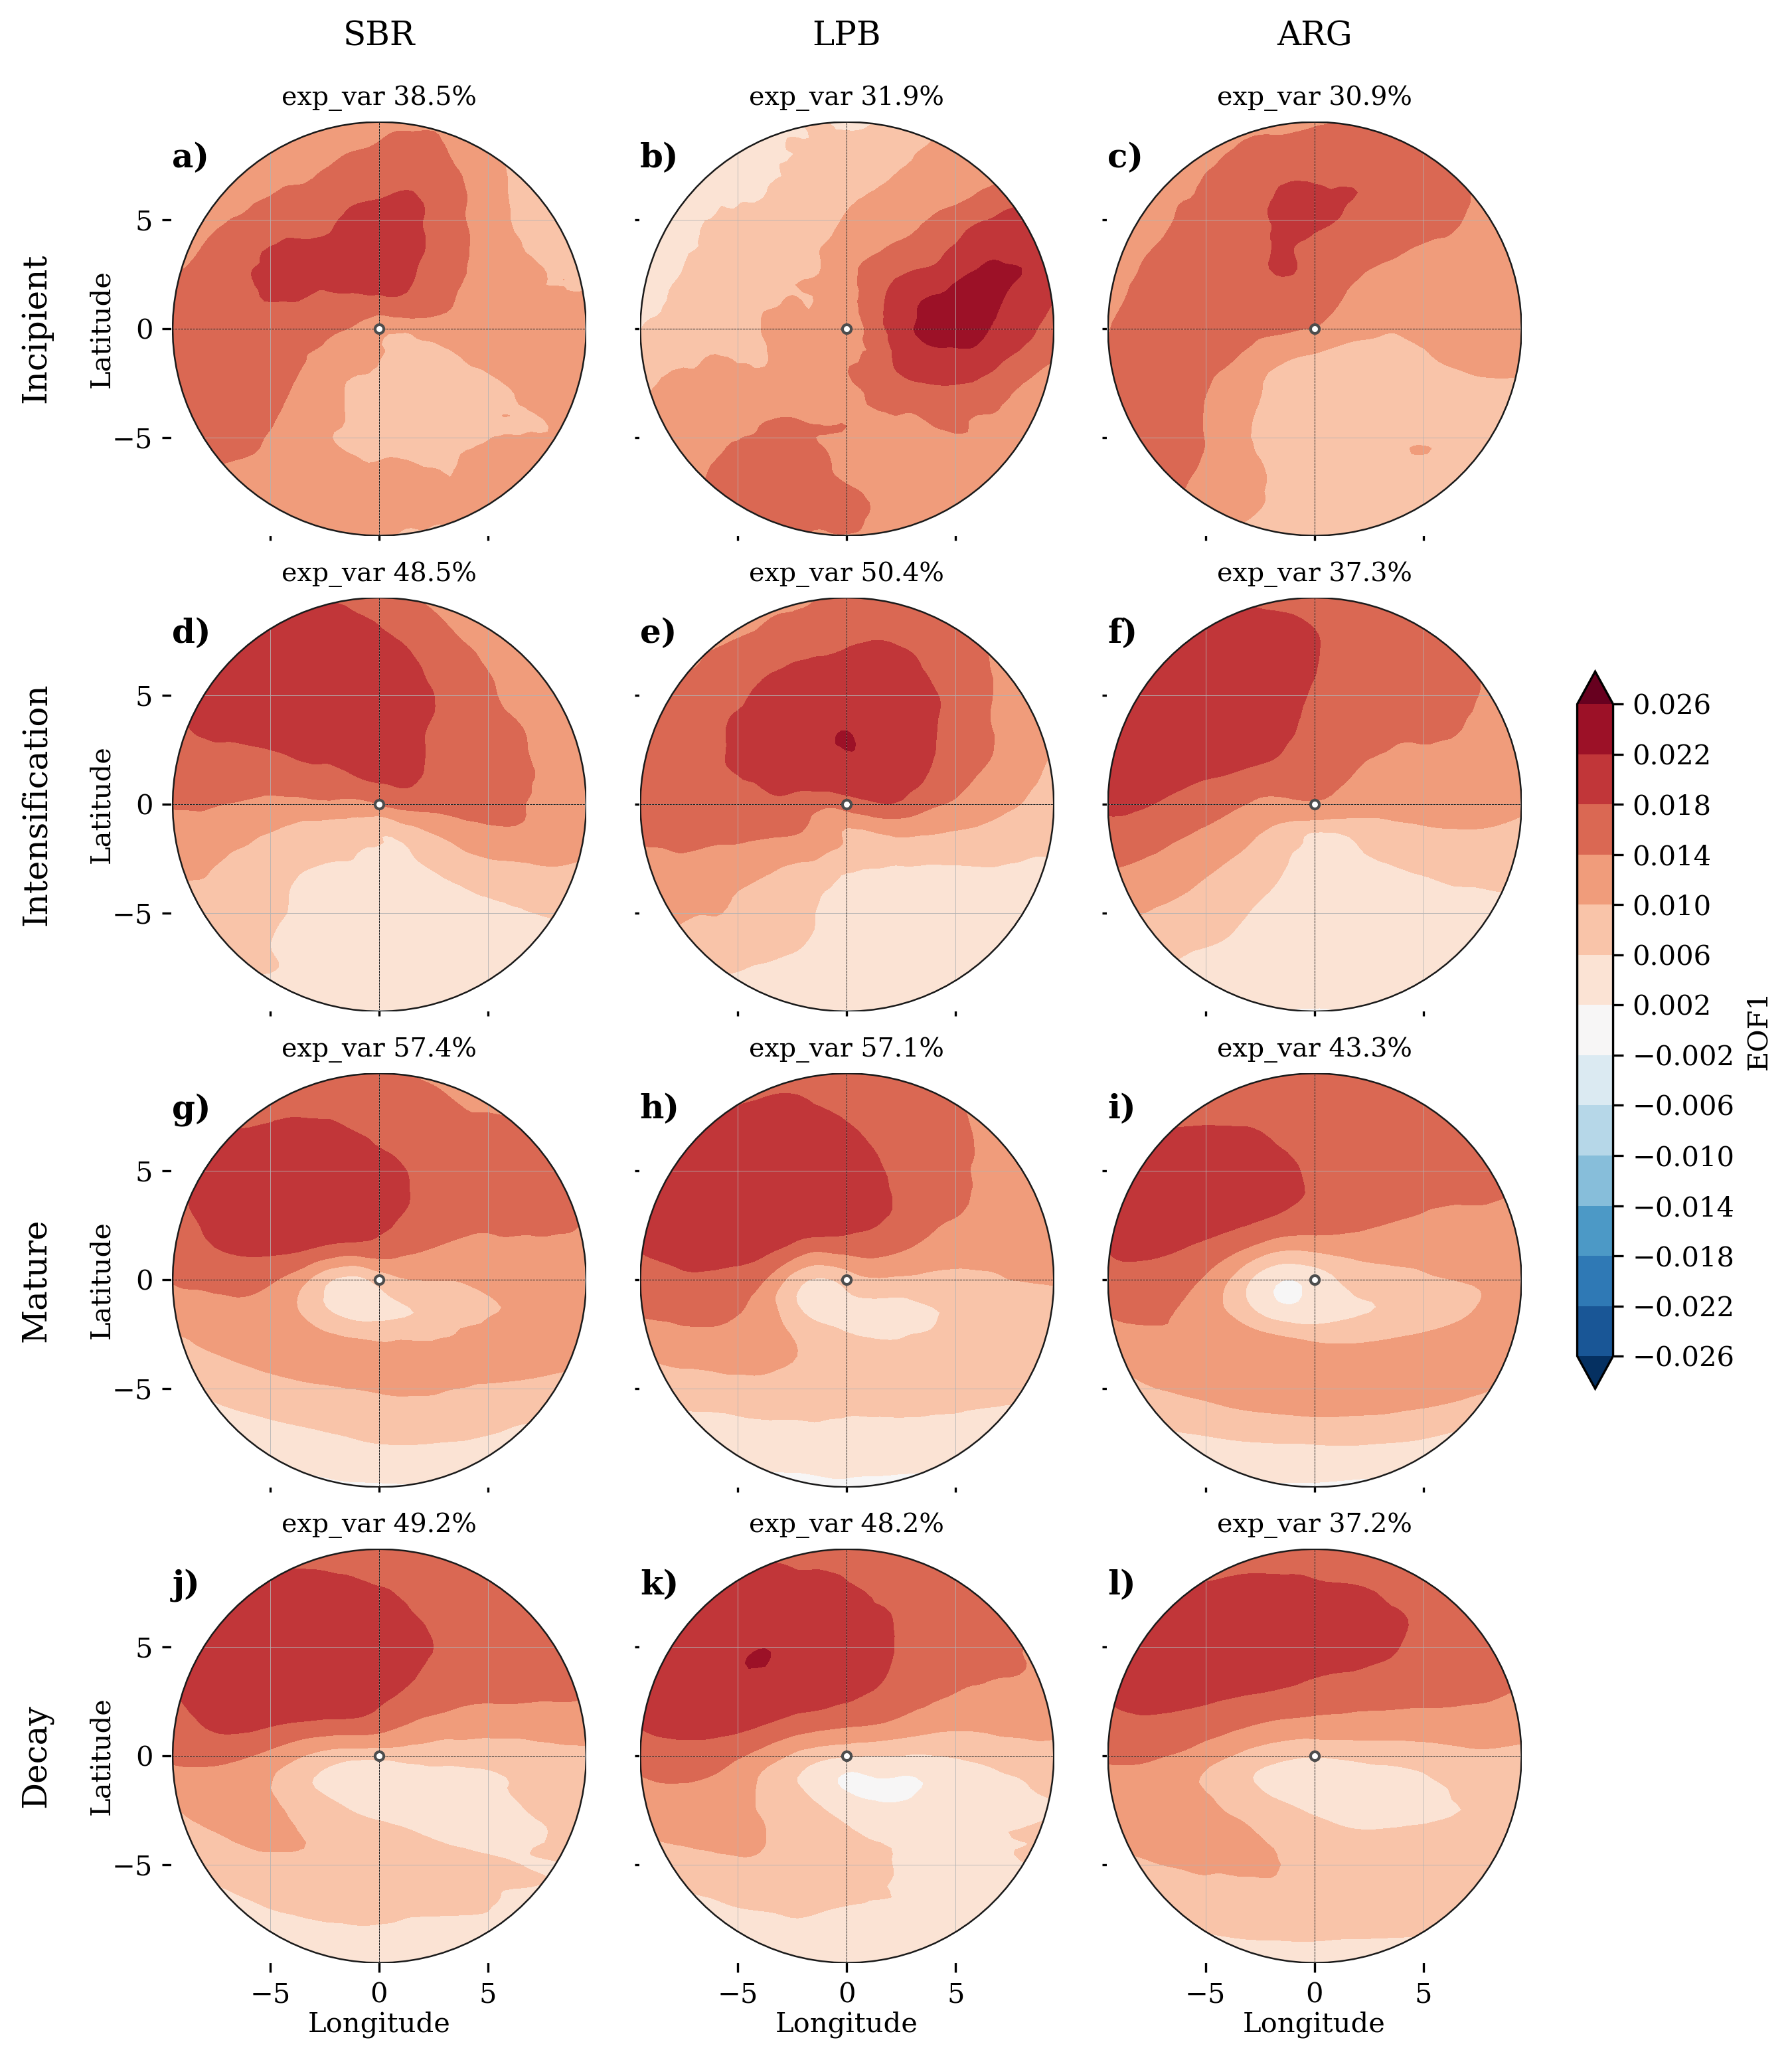
\includegraphics[width=\textwidth]{images/w10/pca1_wind10_global_fasesxreg.png}
\caption[EOF1 de la magnitud del viento a 10 metros - Población Global]{Primer modo espacial (EOF1) de la magnitud del viento a 10 metros para la Población Global de referencia. Los paneles (a-c) corresponden a la fase incipiente (Ic) para las regiones SBR, LPB y ARG, respectivamente; (d-f) a la intensificación (It); (g-i) a la madurez (M); y (j-l) al decaimiento (D). El título de cada panel indica el porcentaje de varianza explicada (\textit{exp\_var}) por este modo dominante. Los colores cálidos (fríos) representan anomalías positivas (negativas) de la estructura del viento relativo al centro del ciclón en un dominio de $20^{\circ} \times 20^{\circ}$.}
\label{fig:eof1_wind10_global}
\end{figure}

La Figura~\ref{fig:eof1_wind10_global} presenta el primer modo de las Funciones Ortogonales Empíricas (EOF1) del campo de viento a 10 metros, obtenido mediante la descomposición de la varianza total espacial sobre el dominio lagrangiano. Tal como se evidenció en el fraccionamiento de energía (Sección~\ref{sec:var_exp_wind10}), el patrón EOF1 global domina ampliamente la varianza del sistema, exhibiendo valores que oscilan entre el 31.9\% y el 57.4\% según la región y fase. Morfológicamente, rige una estructura de gran escala donde las anomal\'ias positivas dominan el cuadrante norte y la periferia del dominio (tonos rojos, $+0.01$ a $+0.02$), mientras que una zona de anomal\'ias negativas o neutras se concentra
alrededor y al sur del centro del v\'ortice (tonos blancos--azules claros). La región LPB en intensificación (e) muestra un patrón morfológicamente distinto, con un núcleo anómalo positivo centralizado. Finalmente, en la fase de decaimiento (j, k, l), el dipolo se homogeneiza y adopta una disposición estrictamente zonal en todas las regiones, separando el dominio en una mitad norte negativa y una mitad sur fuertemente positiva.
% ELIMINADO: Párrafo introductorio previo que definía el análisis como "aplicado sobre Población Global estratificada por región...". 
% RAZÓN: Esta información ya está contenida implícitamente en el caption de la figura y explícitamente en la introducción del capítulo (Sección 5.1), donde se estableció el dominio lagrangiano y la estratificación. Repetirlo aquí interrumpe la progresión argumental desde la sección KDE anterior.

La presencia de este dipolo norte-sur de gran escala, sumado a su alta varianza explicada, indica que la principal fuente de variabilidad en el viento de los ciclones típicos está dictada por su interacción con el flujo zonal de fondo (los vientos del oeste de latitudes medias) y las fluctuaciones del gradiente latitudinal de temperatura. Como detalla \citet{hannachi2007empirical}, la emergencia de una estructura dipolar dominante (EOF1) constituye la firma matemática que representa el desplazamiento posicional de una corriente. Físicamente, en el Hemisferio Sur, esto se traduce en desplazamientos de la latitud relativa de las corrientes en chorro en la alta troposfera. De acuerdo con \citet{hoskins2005new} y \citet{dossantos2023response}, la evolución estructural de los ciclones ordinarios depende fuertemente de este acoplamiento baroclínico profundo; por lo tanto, las anomalías capturadas por la EOF1 reflejan cómo el sistema expande o contrae su campo de viento en respuesta a la posición del chorro. 
% CITA TEXTUAL HANNACHI (2007): "Often, a dipole pattern in the first EOF represents a spatial shift or translation of a dominant atmospheric feature..."
% CITA TEXTUAL HOSKINS (2005) / DOS SANTOS (2023): 

El hecho de que las anomalías positivas de este dipolo se concentren marcadamente al sur del centro (tonos rojos en d, f, g, i) responde a la asimetría térmica característica de los sistemas del Atlántico Sur. Tal como describen \citet{sinclair1997objective} y \citet{reboita2010south}, a medida que los ciclones se intensifican y ganan latitud, el gradiente horizontal de presión tiende a maximizarse en su sector austral (o polar) debido a la interacción de la circulación ciclónica con los anticiclones migratorios, acelerando los vientos en esa franja. 
% CITA TEXTUAL SINCLAIR (1997) / REBOITA (2010):
La excepción geométrica observada en la región LPB (e) durante su intensificación respalda esta dependencia de los forzantes físicos: de acuerdo con \citet{gramcianinov2019properties}, los sistemas en esta zona están fuertemente modulados en sus etapas iniciales por la influencia de la baja orográfica, lo que genera una varianza del viento anclada a forzantes topográficos centralizados, retrasando temporalmente la imposición del dipolo zonal de gran escala. Finalmente, en el decaimiento, cuando la baroclinicidad se agota y el vórtice se debilita, la estructura circulatoria propia del ciclón pierde definición y la variabilidad queda completamente subyugada a los desplazamientos del gradiente de presión meridional del entorno sinóptico subyacente.
% CITA TEXTUAL GRAMCIANINOV (2019): "LA PLATA [LPB] cyclones development is influenced by an orographic low in their early stages..."

La extracción de este patrón univariado cumple la función de establecer la línea base de variabilidad estructural para el ciclón extratropical promedio. Identificar que la fluctuación principal en sistemas ordinarios obedece a un dipolo meridional permite separar matemáticamente las alteraciones inducidas por el entorno de aquellas generadas por la propia dinámica interna del vórtice.
% ELIMINADO: La última oración del párrafo anterior que afirmaba: "Este marco de referencia es instrumental para evaluar si los eventos extremos manifiestan modos espaciales organizativos diferentes o simplemente amplifican la señal de la población media."
% RAZÓN: Esta anticipación de los resultados del grupo p90 (la pregunta de investigación) se traslada directamente al inicio de la siguiente subsección como contraste activo, evitando la duplicidad de funciones entre el cierre de Global y la apertura de p90. Se mantiene la idea de "línea base" pero se elimina la pregunta retórica que se responderá inmediatamente después.

\subsubsection{Subconjunto p90}\label{subsubsec:eof1_wind10_p90}

\begin{figure}[htbp]
\centering
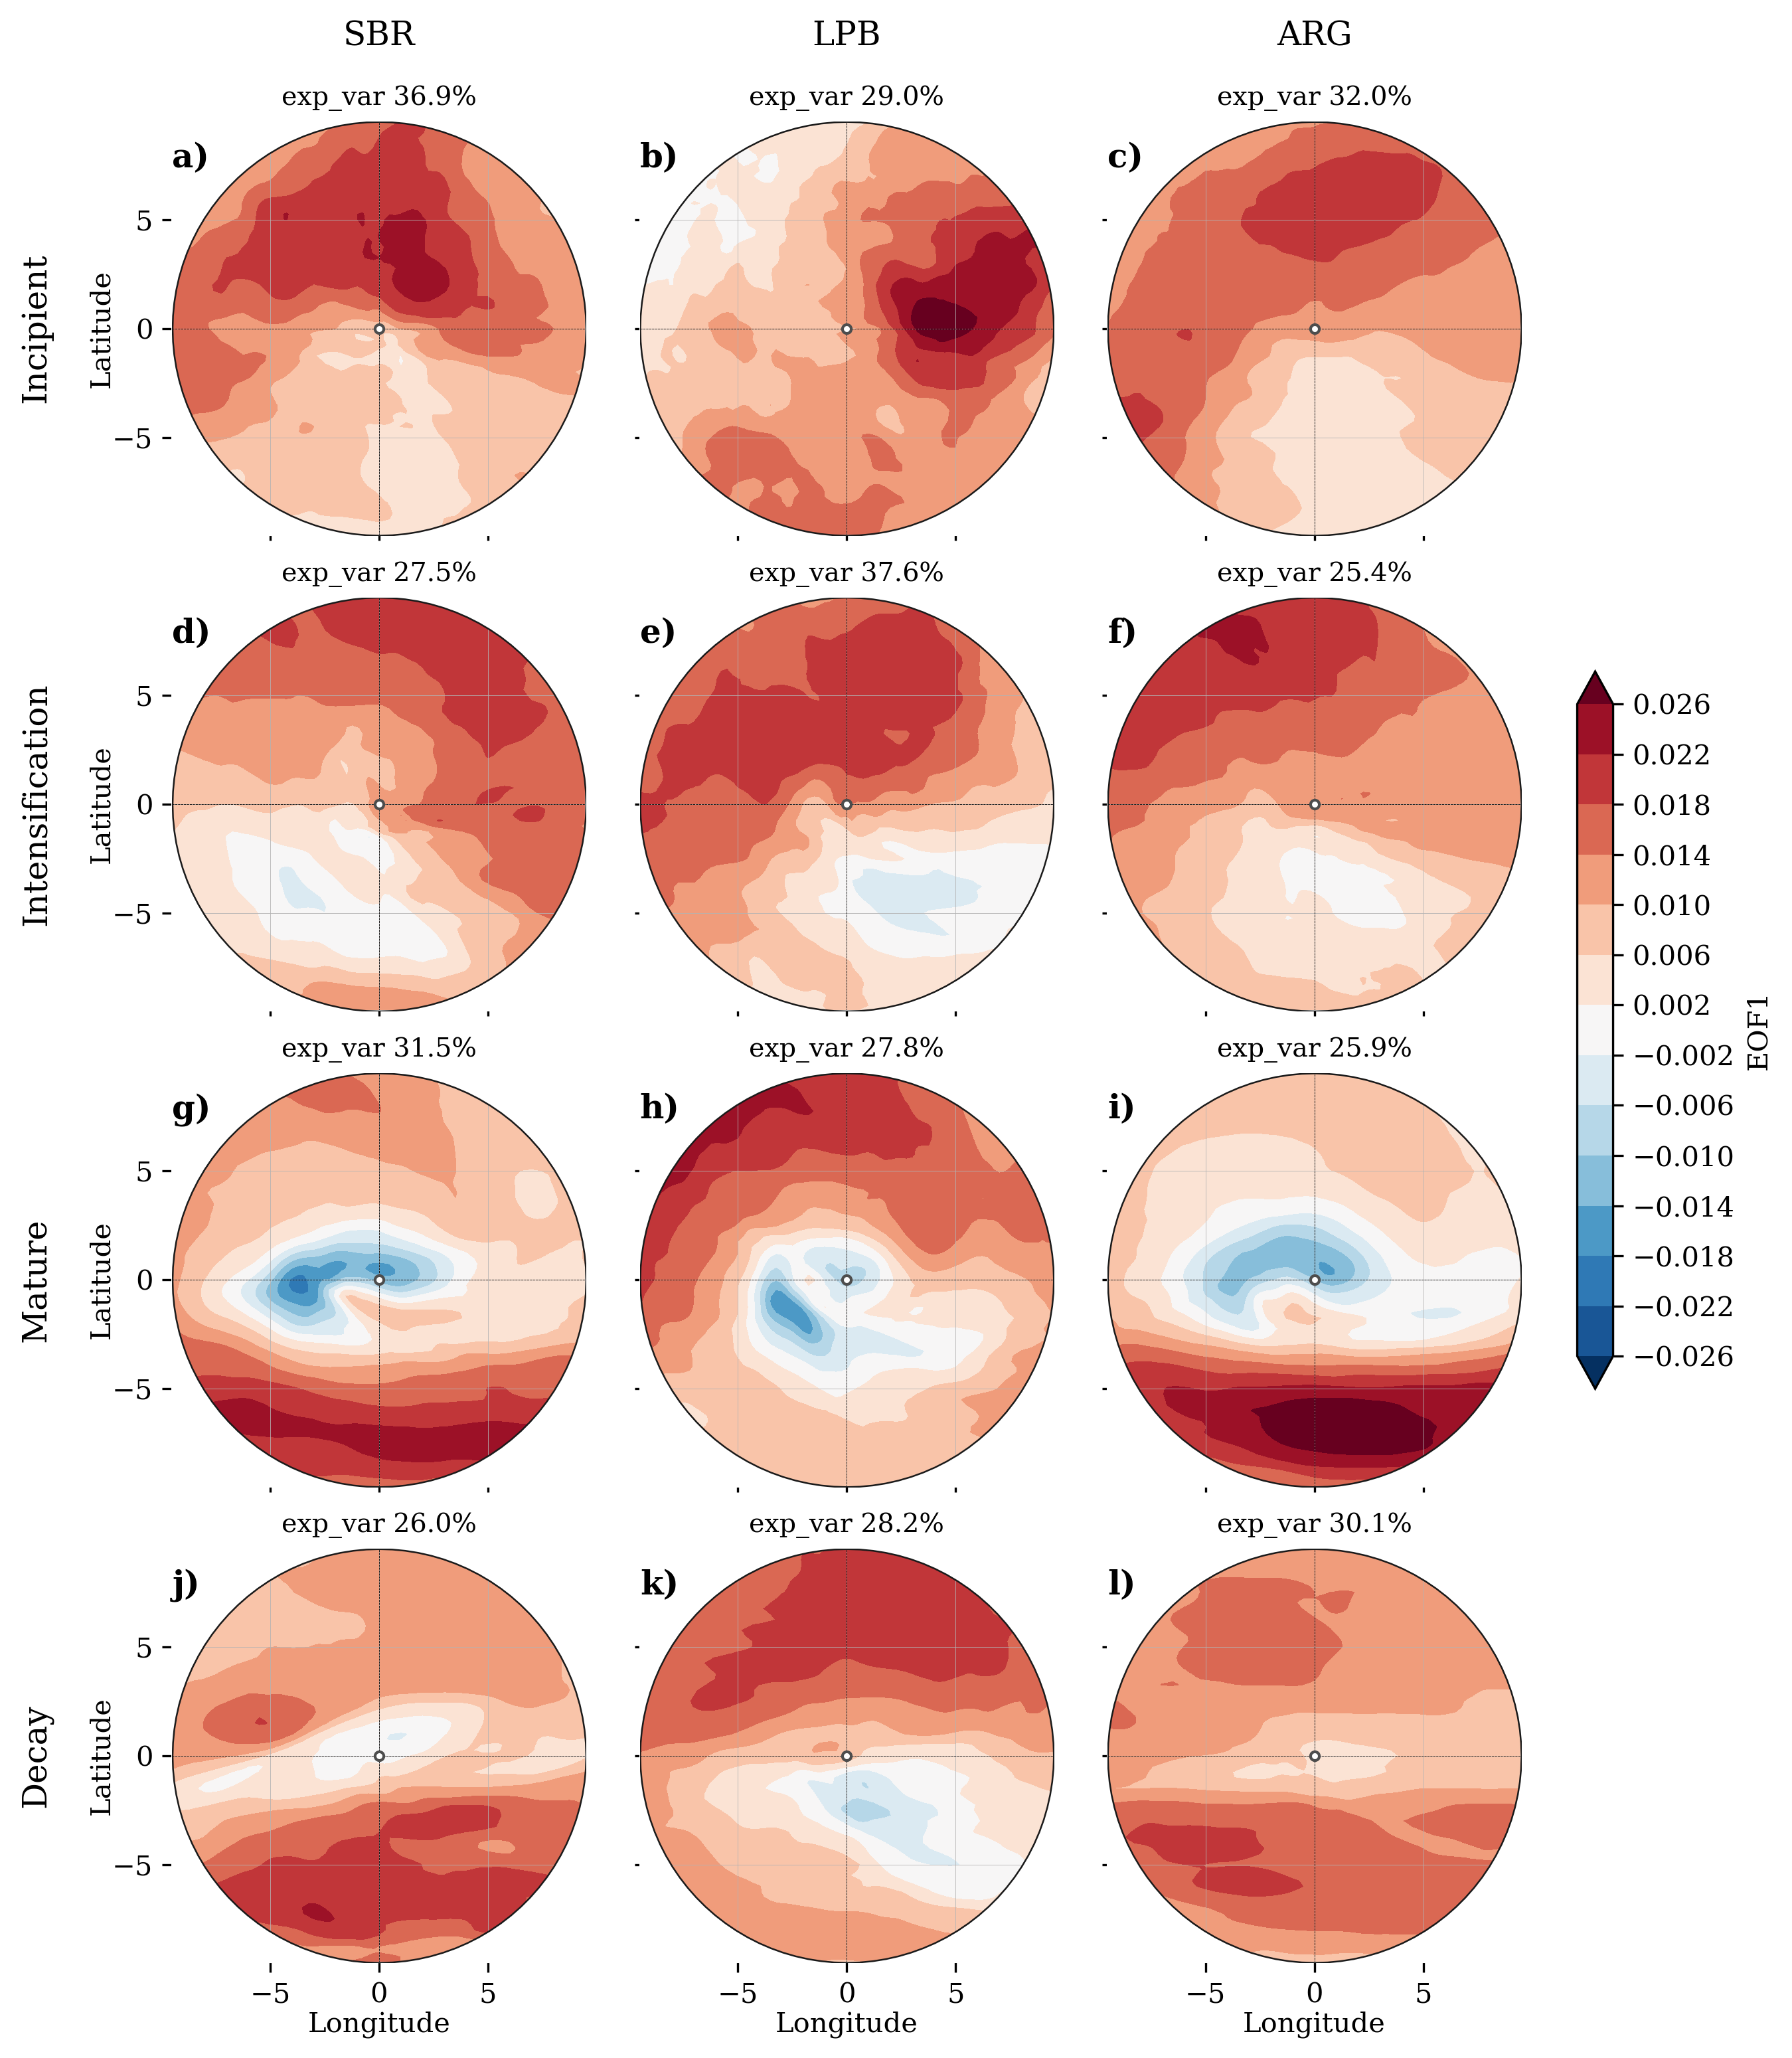
\includegraphics[width=\textwidth]{images/w10/pca1_wind10_p90_fasesxreg.png}
\caption[EOF1 de la magnitud del viento a 10 metros - Subconjunto p90]{Primer modo espacial (EOF1) de la magnitud del viento a 10 metros para el subconjunto de ciclones intensos (p90). La disposición de los paneles (a-l) por región de ciclogénesis (columnas) y fase evolutiva (filas) es idéntica a la Figura~\ref{fig:eof1_wind10_global}. Se detalla la varianza explicada (\textit{exp\_var}) en cada panel y la barra de color estandarizada para evaluar las diferencias en las firmas espaciales de los eventos extremos frente al comportamiento climatológico.}
\label{fig:eof1_wind10_p90}
\end{figure}

El contraste contra la organización dipolar de la población general revela que los ciclones extremos no amplifican linealmente el patrón base, sino que reconfiguran radicalmente su arquitectura modal. La Figura~\ref{fig:eof1_wind10_p90} ilustra que, en el estrato p90, la proporción de energía capturada por el modo EOF1 se reduce drásticamente, oscilando entre el 25.4\% y el 37.6\%, y su topología difiere sustancialmente al mostrar firmas espacialmente complejas e hiperlocalizadas. En la fase de intensificaci\'on de SBR (d), emerge una fuerte
anomal\'ia positiva que cubre la mayor parte del dominio, con mayor intensidad en el norte y noroeste (rojo oscuro, $>+0.03$). Más destacable es el comportamiento en madurez (g, h, i): LPB (h) exhibe un dipolo fuertemente inclinado con un n\'ucleo negativo sumamente intenso y compacto al sur del centro, rodeado por una regi\'on de anomal\'ias positivas que domina el sector norte y noroeste del dominio; ARG (i) desarrolla un patr\'on complejo donde la anomal\'ia positiva cubre el norte y la periferia sur, con una regi\'on de transici\'on en el centro. En el decaimiento (j, k, l), aunque retorna una estructura pseudozonal, los gradientes anómalos son notablemente más estrechos y confinados cerca del núcleo en comparación con la relajación expansiva observada en la población general.
% ELIMINADO: Párrafo introductorio que definía: "Este análisis descompone el campo de viento... para aislar las fluctuaciones dominantes en los sistemas que... registraron los mínimos absolutos de vorticidad dentro del primer decil...".
% RAZÓN: La definición del grupo p90 (percentil 90, vorticidad mínima) ya fue establecida en la introducción del capítulo (Sección 5.1) y reafirmada implícitamente en la sección KDE (5.2.2). Re-definirlo aquí genera una "introducción de introducción". El salto directo al contraste ("El contraste contra...") activa inmediatamente la comparación prometida por el cierre de la subsección Global anterior.

La quiebra del patrón dipolar simple y la hiperlocalización de las anomalías son la manifestación espacial de la fragmentación de energía multiescalar discutida previamente. Físicamente, esto confirma que en los eventos extremos la intensa circulación cerrada de mesoescala domina sobre el flujo de fondo. El núcleo compacto y potente observado en la madurez de LPB (h) evidencia variabilidad en la posición exacta y severidad de estructuras mesoescalares. De acuerdo con el marco dinámico documentado por \citet{clark2005sting} y \citet{han2025system} —y coherente con la localización espacial discutida en la Sección~\ref{sec:kde_espacial_p90}—, la cinta transportadora fría (\textit{cold conveyor belt}) y los procesos de fractura frontal rápida impulsados por altas tasas de vorticidad se traducen modalmente en un EOF1 compacto y localizado, incapaz de capturarse mediante un patrón de gran escala. Por otro lado, en ARG (i), la aparición de un patrón tripolar con una anomalía negativa central durante la madurez indica fluctuaciones en el tamaño o intensidad del "ojo" o seclusión cálida (\textit{warm seclusion}). Como detallan \citet{schultz2021antecedents} y \citet{reboita2022from}, la formación de esta seclusión cálida en el núcleo, rodeada por un anillo de vientos huracanados, es el rasgo evolutivo culminante del modelo conceptual de Shapiro-Keyser, una vía de desarrollo característica de ciclones con alta organización baroclínica y fuerte interacción con flujos anómalos en altas latitudes.
% CITA TEXTUAL CLARK (2005) / HAN (2025): 
% CITA TEXTUAL SCHULTZ (2021) / REBOITA (2022): "The Shapiro-Keyser cyclone model... features a wrapping around of the bent-back front to form a warm-core seclusion of post-cold-frontal air."

La cuantificación de estos modos revela una conclusión central: un ciclón extremo no es equivalente a un ciclón ordinario escalado linealmente, sino que su severidad dinámica modifica de raíz la arquitectura del sistema. Como enfatizan \citet{corner2025classification} y \citet{eisenstein2023identification}, la severidad del viento no depende únicamente de la profundidad sinóptica, sino de la manifestación de estas características mesoescalares. Identificar estas firmas asimétricas y compactas es clave para la meteorología operativa aplicada, ya que demuestra que la variabilidad de los vientos más destructivos se rige por procesos internos al vórtice, lo cual exige modelos de pronóstico capaces de resolver la dinámica estructural fina en los cuadrantes inmediatos al centro del ciclón.

% ==============================================================================
% ==============================================================================

\subsection{Significancia estadística}\label{subsec:res_significancia_madurez}
% ==============================================================================
%\subsection{Significancia espacial de los patrones en la fase de madurez}\label{subsec:res_significancia_madurez}

Para discriminar entre señales físicas robustas y fluctuaciones estocásticas propias del remuestreo, se evaluó la significancia estadística de los autovectores espaciales mediante el método Bootstrap-$t$ (Sección \ref{subsec:bootstrap_significancia}). La Figura \ref{fig:xeof_madurez_global} documenta los tres primeros modos (EOF1--EOF3) y sus respectivas series temporales (PC1--PC3) para la Población Global en fase de madurez, mientras que la Figura \ref{fig:xeof_madurez_p90} presenta el análisis equivalente para el subconjunto extremo (p90). El achurado ($\backslash\backslash\backslash$) delimita las áreas donde las cargas espaciales resultaron estadísticamente significativas al 95\% de confianza.

\begin{figure}[htbp]
\centering
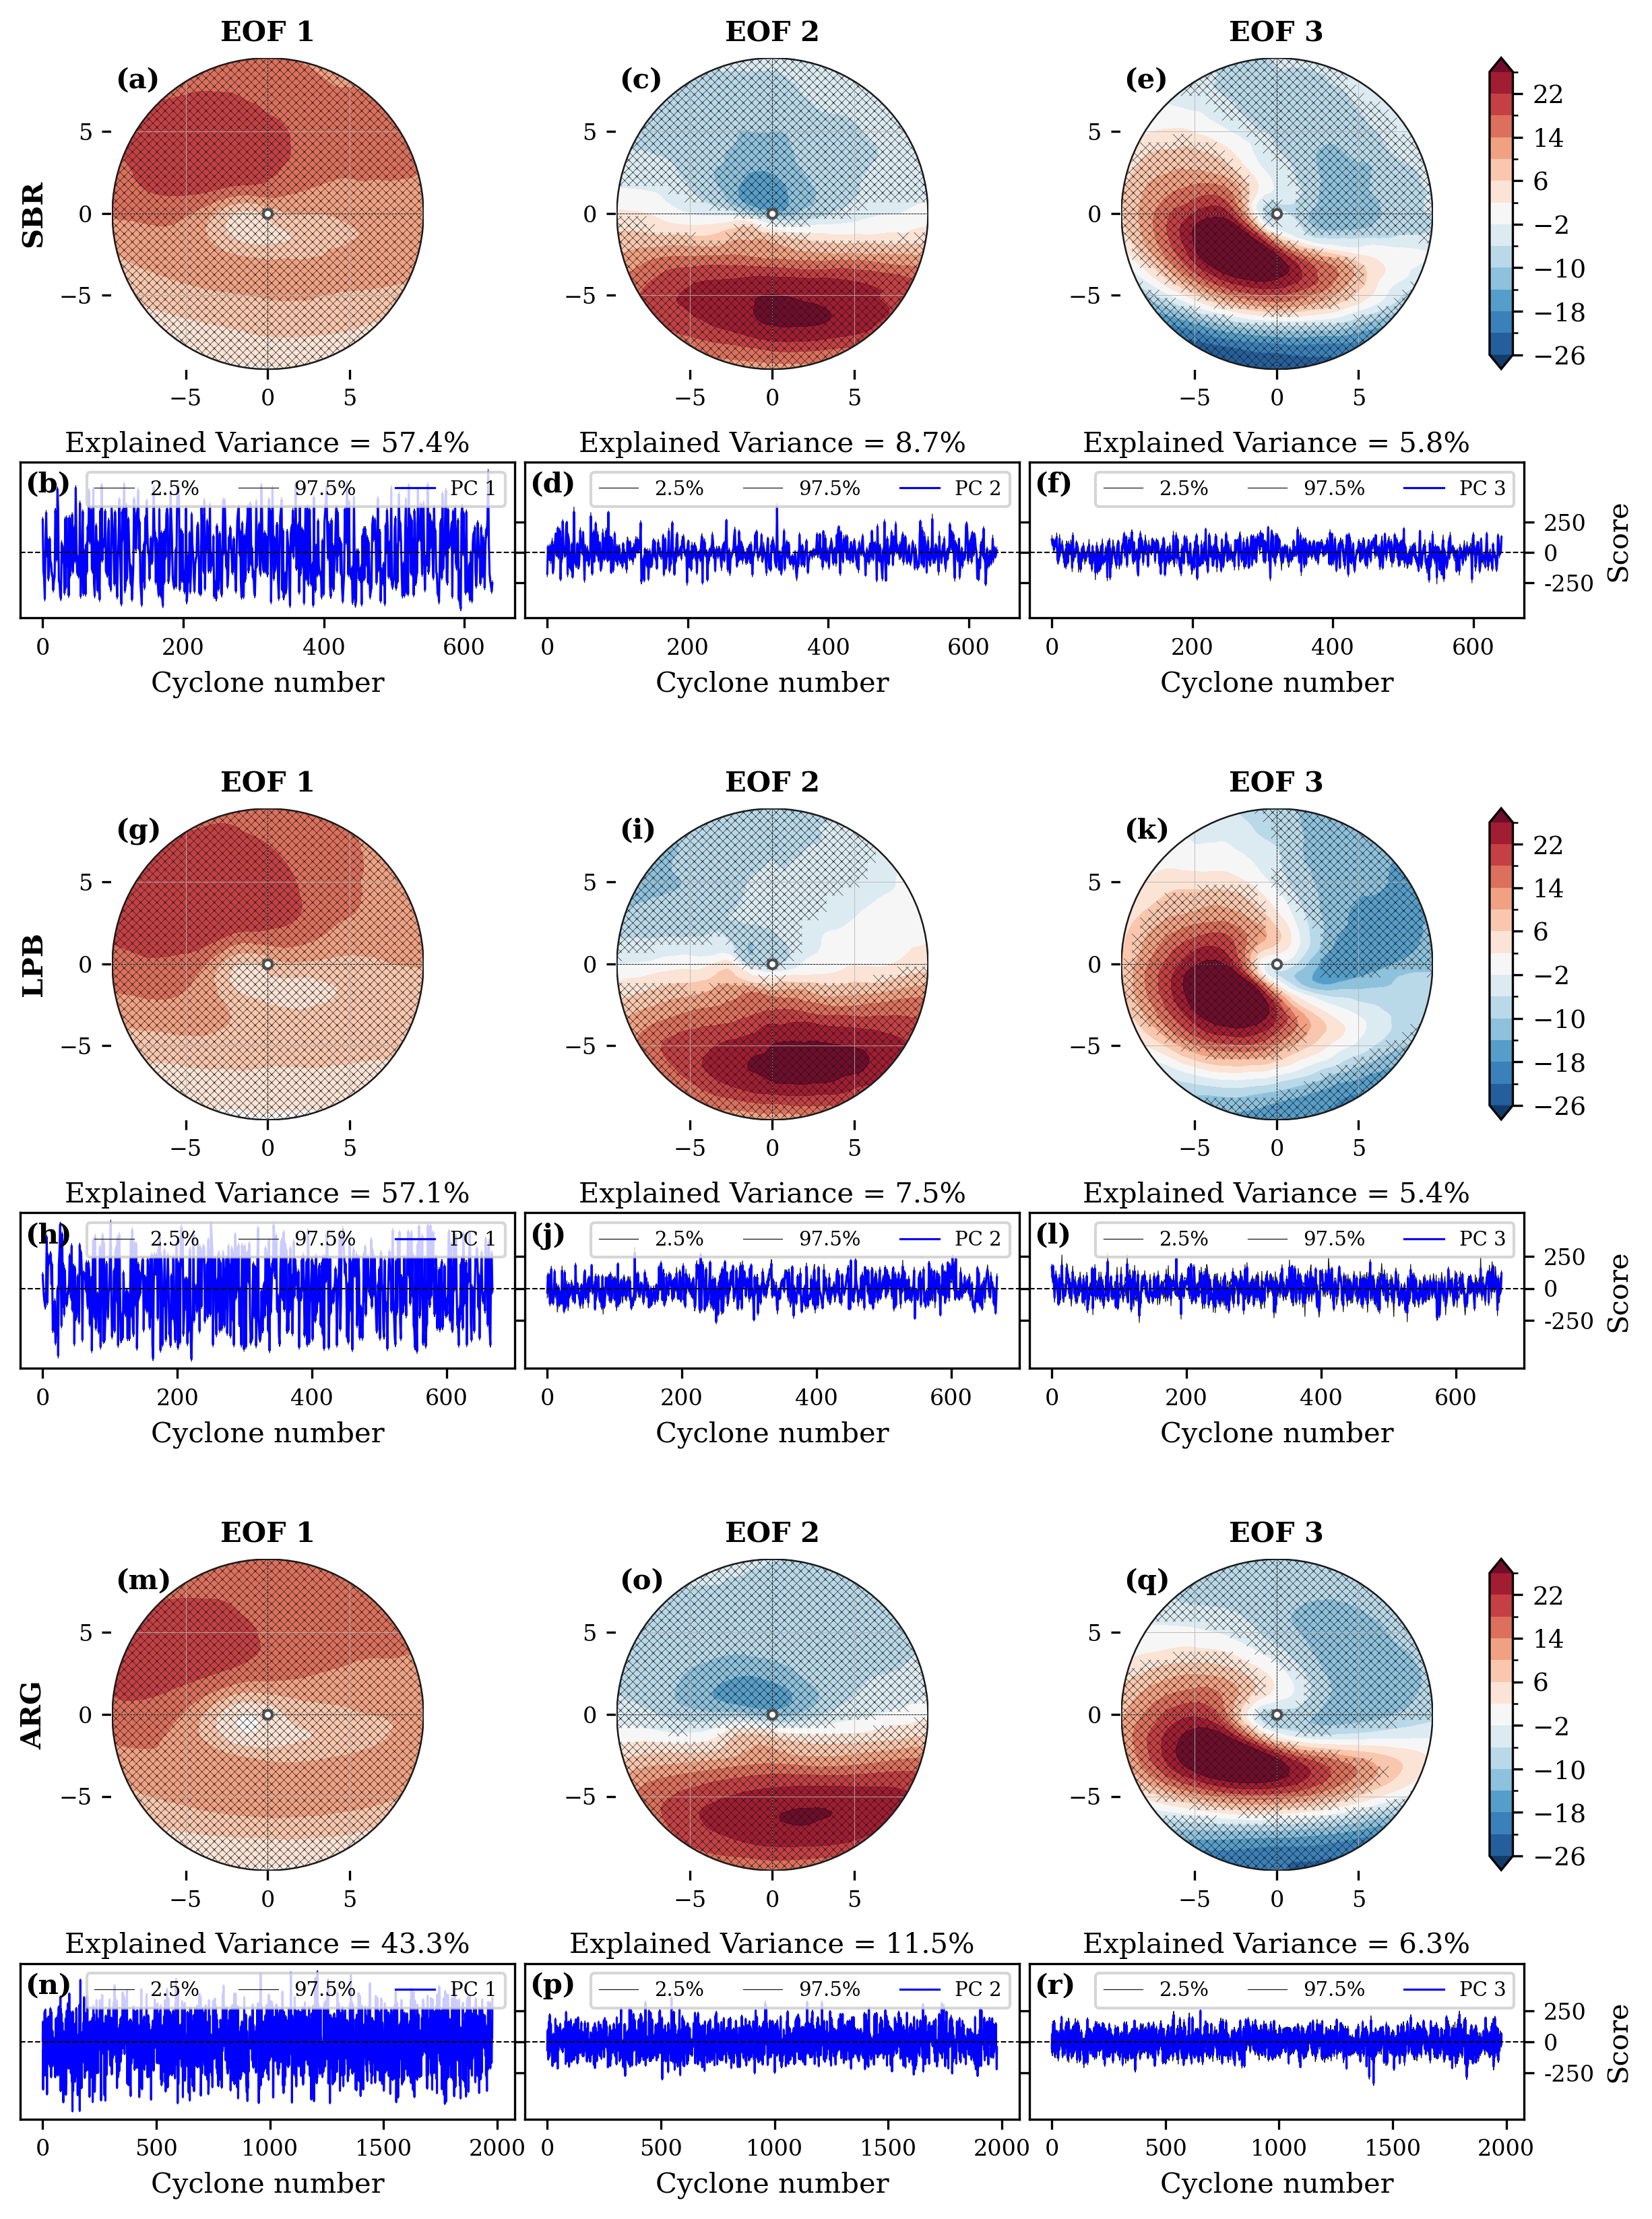
\includegraphics[width=\textwidth]{images/w10/xeof_global_wind10_mature.png}
\caption[Significancia espacial de los EOFs en fase de madurez - Población Global]{Descomposición EOF del viento a 10 m para la Población Global en fase de madurez. Paneles (a, c, e): mapas de los tres primeros modos espaciales (EOF1--EOF3) con achurado indicando significancia estadística al 95\% (test Bootstrap-$t$). Paneles (b, d, f): series temporales correspondientes de las Componentes Principales (PC1--PC3). La línea gris delimita los percentiles 2.5 y 97.5 de la distribución bootstrap.}
\label{fig:xeof_madurez_global}
\end{figure}

\begin{figure}[htbp]
\centering
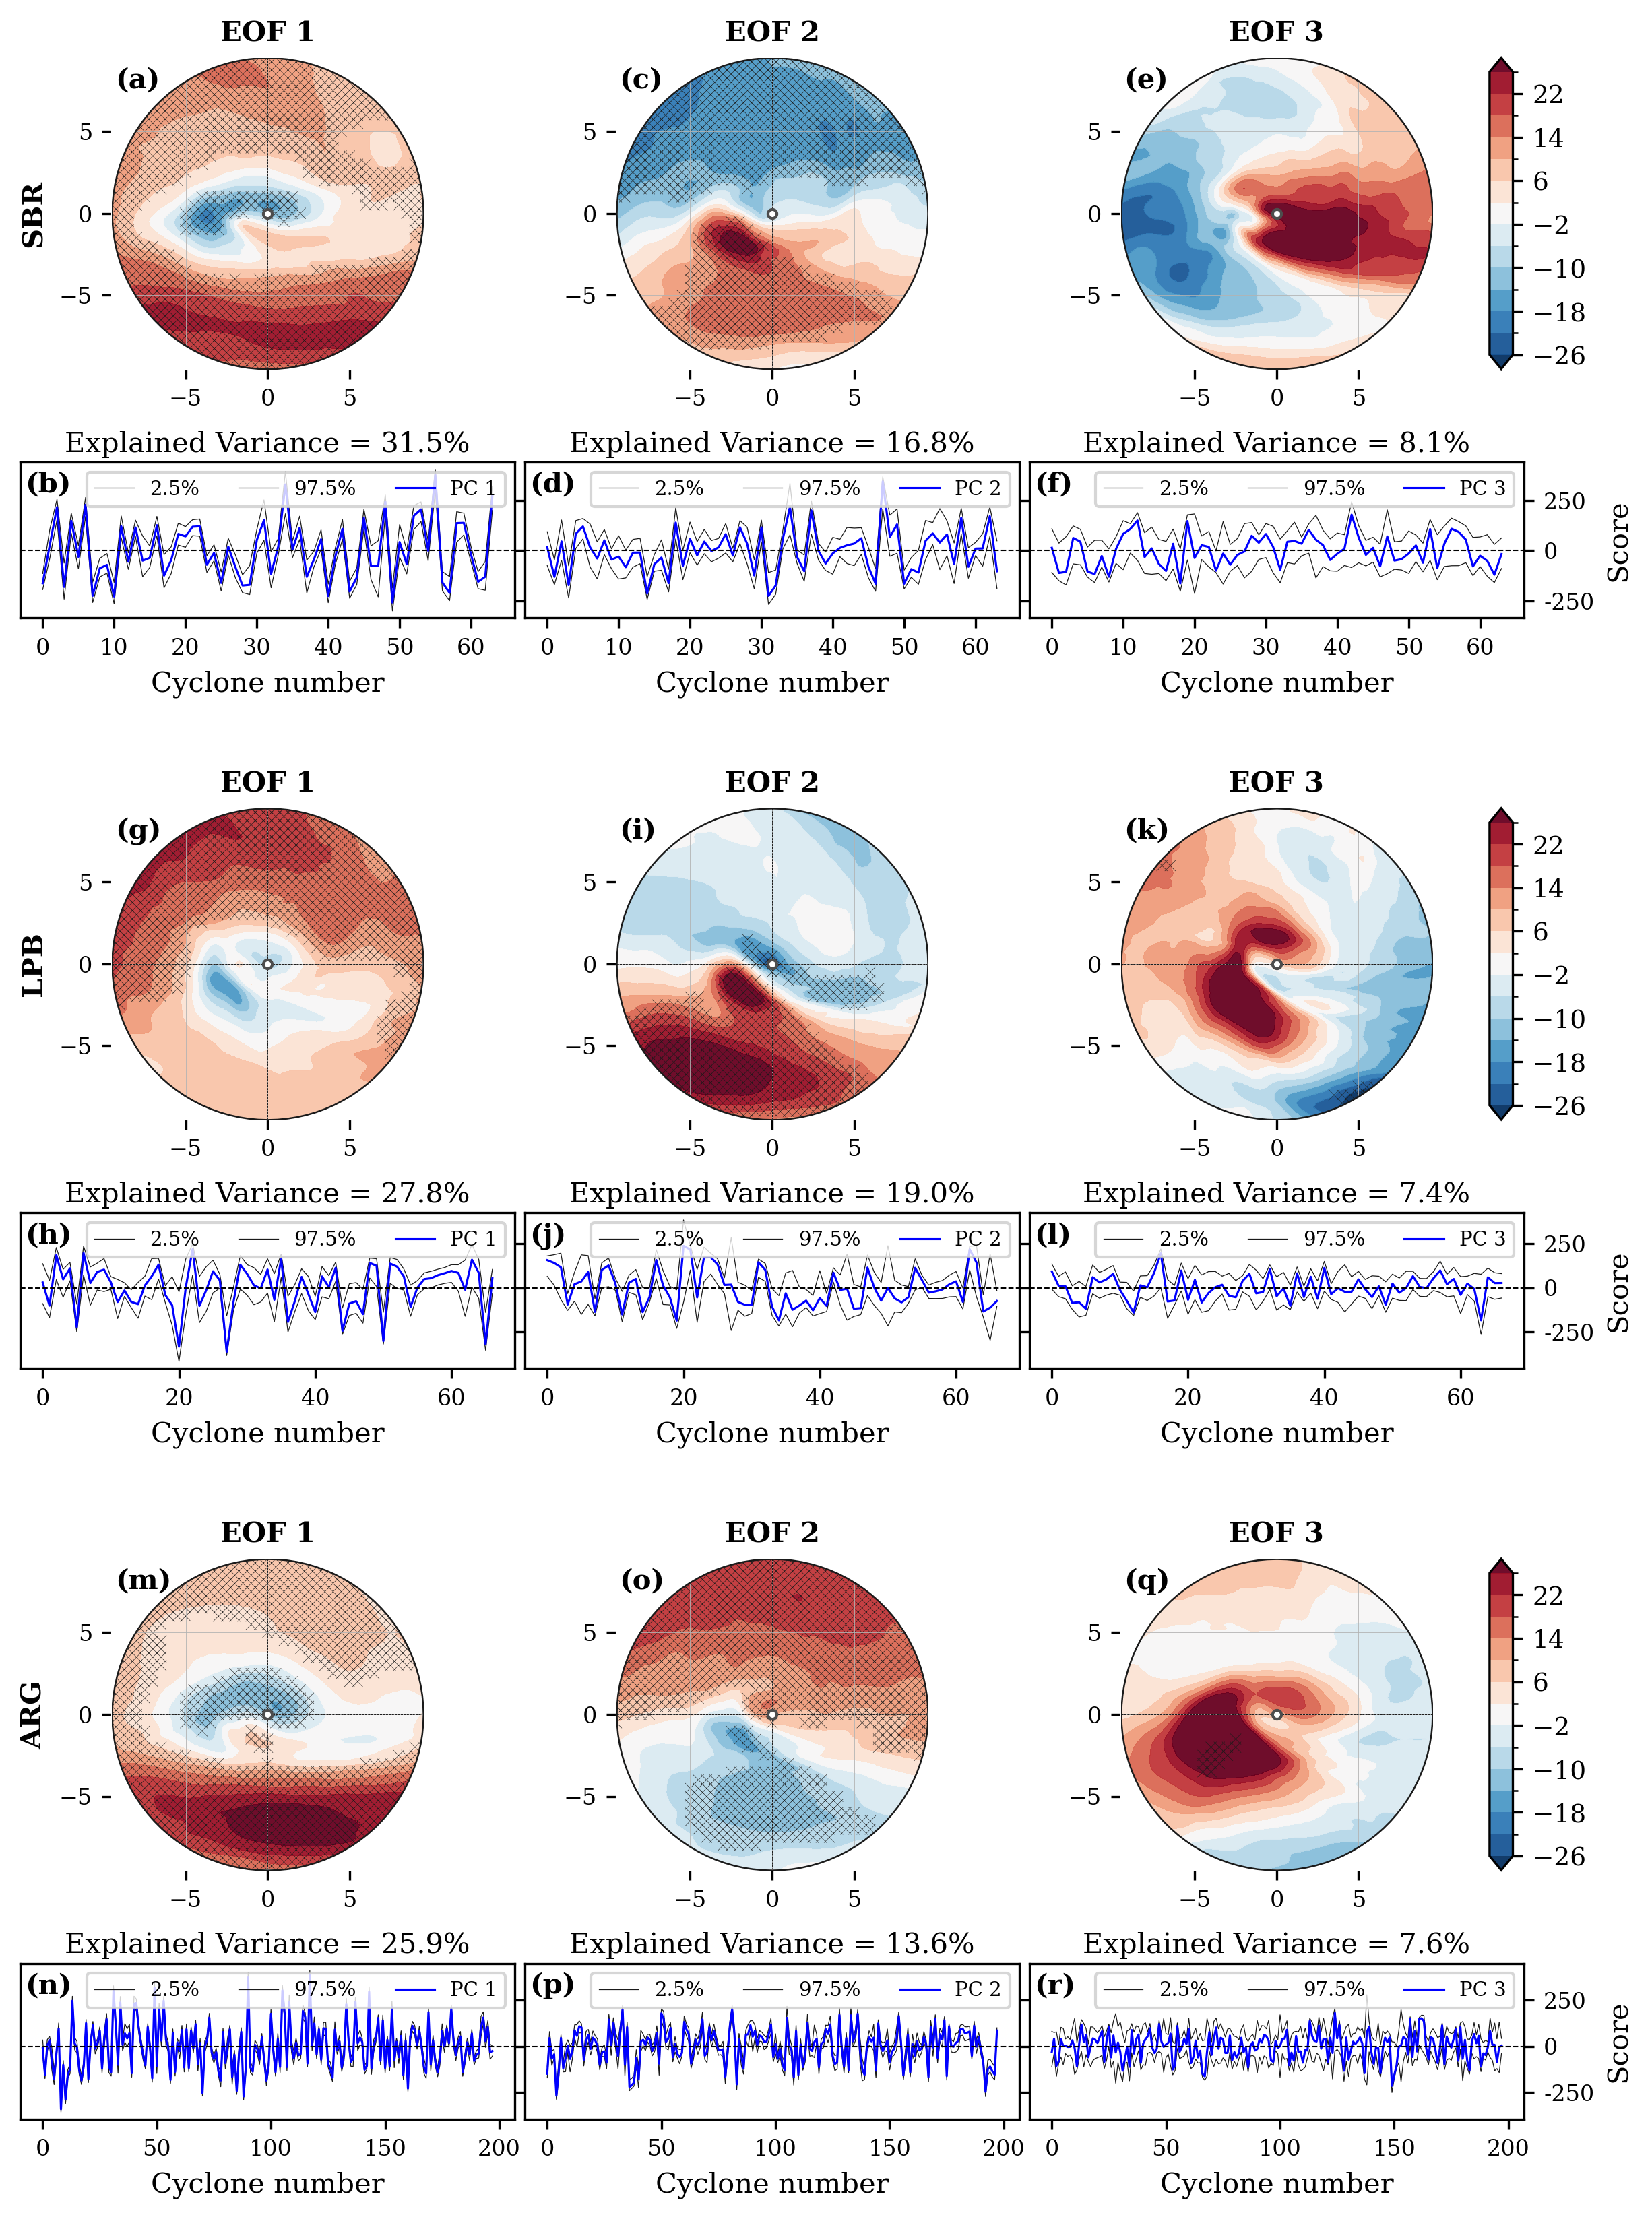
\includegraphics[width=\textwidth]{images/w10/xeof_p90_wind10_mature.png}
\caption[Significancia espacial de los EOFs en fase de madurez - Subconjunto p90]{Descomposición EOF del viento a 10 m para el subconjunto extremo (p90) en fase de madurez. La disposición de paneles es idéntica a la Figura \ref{fig:xeof_madurez_global}.}
\label{fig:xeof_madurez_p90}
\end{figure}

En la Población Global (Figura \ref{fig:xeof_madurez_global}), el modo dominante (EOF1) exhibe áreas de significancia estadística que abarcan prácticamente todo el dominio, particularmente en los sectores norte y sur donde se localizan los máximos del dipolo baroclínico (paneles a, g, m). Esta extensión espacial de la significancia indica que el patrón dipolar no es un artefacto de la muestra, sino una característica física estable y reproducible de los ciclones maduros. Consistente con el alto porcentaje de varianza explicada (43--57\%), las series de PC1 (paneles b, h, n) muestran amplitudes que oscilan ampliamente y dominan sobre las fluctuaciones de PC2 y PC3, las cuales permanecen confinadas dentro de los límites de confianza (líneas grises) y representan meramente ruido de fondo o variabilidad intra-sistémica menor.

Por el contrario, en el subconjunto extremo (Figura \ref{fig:xeof_madurez_p90}), las áreas significativas del EOF1 experimentan una dramática contracción hacia núcleos compactos próximos al centro del vórtice (paneles a, g, m). En SE-BR y LPB, la significancia se restringe a pequeños parches alrededor del núcleo y el flanco sur, mientras que en ARG el patrón tripolar presenta significancia únicamente en el anillo periférico sur. Esta contracción espacial confirma que, en ciclones intensos, el modo dominante pierde coherencia espacial fuera del núcleo inmediato; la estructura del viento ya no está gobernada por un gradiente sinóptico extendido, sino por procesos de mesoescala localizados (seclusiones térmicas, jets de bajo nivel) que varían sustancialmente entre eventos individuales.

Más crítico aún es el comportamiento de las series temporales en el grupo p90 (paneles b, d, f y h, j, l). A diferencia del grupo Global donde PC2 y PC3 son residuales, aquí las amplitudes de PC2 (l\'inea azul en paneles d, j) y PC3 (paneles f, l) presentan magnitudes comparables a las de PC1 y con frecuencia superan los l\'imites de confianza del 95\%, cruzando los límites de confianza de manera sistemática. Esto demuestra estadísticamente que los modos secundarios han dejado de ser ``ruido'' para convertirse en portadores de varianza física significativa. La competencia energética entre múltiples PCs refleja la fragmentación dinámica del campo de viento: cuando un ciclón alcanza severidad extrema, su estructura cinemática ya no puede describirse mediante un único patrón espacial dominante, sino que requiere la superposición de varios modos ortogonales competitivos.

La implicación meteorológica es profunda. La contracción de las áreas significativas en el grupo p90 indica que la predictibilidad espacial del campo de viento se reduce drásticamente en ciclones extremos. Mientras que en sistemas ordinarios podemos confiar en que el patrón dipolar extendido representará fielmente la distribución de vientos (alta significancia espacial), en sistemas severos solo el núcleo inmediato del vórtice presenta una señal robusta; los flancos y cuadrantes periféricos están dominados por variabilidad estocástica o estructuras transitorias de mesoescala que escapan al primer modo. Esto valida la necesidad de incluir EOF2 y EOF3 en cualquier reconstrucción o pronóstico de campos de viento para ciclones intensos, ya que el primer modo por sí solo ya no captura adecuadamente la estructura física del sistema.

% ==============================================================================
% ==============================================================================
% ==============================================================================
% ------------------------------------------------------------------------------
\section{Componentes principales (PC1)}\label{subsec:res_dinamica_pc1}
%\subsection{Dinámica de las amplitudes modales (PC1)}\label{subsec:res_dinamica_pc1}
% ------------------------------------------------------------------------------

La fragmentación de la varianza y la contracción de las áreas significativas observadas en la fase de madurez (Sección \ref{subsec:res_significancia_madurez}) tienen su contraparte temporal en el comportamiento estadístico de las Componentes Principales. Mientras que en la Población Global la PC1 domina establemente la evolución del sistema —evidenciado por sus amplitudes superiores y áreas significativas extensas—, en los ciclones extremos la competencia entre múltiples modos ortogonales (Figura \ref{fig:xeof_madurez_p90}) se traduce en propiedades estadísticas distintivas: una correlación débil con el forzante sinóptico y distribuciones de probabilidad con colas pesadas.

\input{tabelas_es/tab_momentos_global_w10.tex}

\subsubsection{Población Global: Convergencia hacia el patrón sinóptico dominante}

Las Tablas \ref{tab:momentos_global_w10} y \ref{tab:corr_global_w10} documentan las métricas estadísticas de la PC1 para la Población Global. Al evaluar la evolución de la población media, la distribución de la PC1 exhibe una progresiva \textit{normalización} estructural. En las tres regiones (SE-BR, LPB y ARG), los valores de curtosis oscilan de forma consistente entre $-0.30$ y $-1.03$ durante la intensificación y madurez, evidenciando distribuciones platicúrticas sin colas extremas dominantes. Notablemente, el régimen transicional de LPB muestra la mayor variabilidad inicial (skewness $+0.99$, leptocurtosis $+1.32$ en fase incipiente), mientras que SE-BR y ARG presentan poblaciones más homogéneas desde etapas tempranas.

El rasgo evolutivo más contundente emerge en el acoplamiento con la vorticidad: en todas las regiones, la correlación inicial —que oscila entre $-0.35$ (LPB) y $-0.57$ (SE-BR)— experimenta un \textit{fortalecimiento sistemático} hasta alcanzar su máximo en la madurez ($-0.890$ en SE-BR, $-0.868$ en LPB y $-0.860$ en ARG), cayendo levemente durante el decaimiento ($\rho < -0.75$).

\input{tabelas_es/tab_corr_global_w10.tex}

Este acoplamiento casi lineal (que explica hasta $r^2 \approx 0.79$ de la varianza en SE-BR) demuestra que, en los ciclones ordinarios, la variabilidad espacial del viento está gobernada directamente por el gradiente de presión a escala sinóptica. La progresiva simetrización de la distribución de PC1 (skewness tendiendo a cero) evidencia que, a medida que el vórtice se intensifica, los campos de viento convergen hacia una configuración prototípica, dominada por el primer modo de variabilidad. Entonces, para la mayoría de los ciclones, la estructura espacial del viento no es arbitraria, sino que se organiza en torno a un patrón coherente (EOF1). La severidad extrema rompe dicha organización, permitiendo que el sistema explore múltiples configuraciones espaciales válidas.

La diferencia entre regiones reside en la velocidad de esta convergencia: mientras SE-BR exhibe un acoplamiento fuerte desde etapas incipientes, LPB requiere la fase de intensificación para alcanzar dicho estado (pasando de $\rho = -0.35$ a $-0.71$), reflejando su carácter transicional donde la organización frontal emerge solo cuando el forzante baroclínico se establece con suficiente intensidad.

Establecer esta línea base cinemática es importante para validar estadísticamente que los modelos de gran escala representan la mayoría de los ciclones. En sistemas de intensidad regular, es posible inferir con alta confianza la magnitud espacial de la circulación superficial observando únicamente la vorticidad relativa en 850 hPa.

\subsubsection{Subconjunto Extremo (p90): Desacoplamiento estructural y bifurcación dinámica}

Las Tablas \ref{tab:momentos_p90_w10} y \ref{tab:corr_p90_w10} exponen los parámetros estadísticos para grupo de ciclones más intensos (p90). La dinámica de los eventos extremos rompe drásticamente con la linealidad observada en la climatología. En lugar de intensificarse hacia la madurez, la correlación entre PC1 y vorticidad exhibe un colapso estructural en las regiones baroclínicas: en ARG cae progresivamente desde $-0.43$ (incipiente) hasta un mínimo de $-0.26$ en madurez, mientras que LPB y SE-BR muestran correlaciones estancadas o en descenso ($-0.37$ y $-0.44$, respectivamente). 

Este colapso correlacional es consistente con la pérdida de significancia espacial observada en el modo dominante (Figura \ref{fig:xeof_madurez_p90}, paneles a, g, m): cuando el patrón espacial solo es robusto en el núcleo inmediato del vórtice pero no en los flancos (como documentó el test Bootstrap-$t$ en la sección anterior), su amplitud temporal (PC1) deja de escalar coherentemente con la intensidad ($\zeta_{850}^{min}$).

\input{tabelas_es/tab_momentos_p90_w10.tex}

Paralelamente, las distribuciones de probabilidad revelan una \textit{heterogeneización} marcada. LPB exhibe leptocurtosis ($\gamma_2 = +0.96$) y fuerte asimetría negativa ($\gamma_1 = -0.88$) durante la intensificación, indicando una población bimodal de configuraciones estructurales. SE-BR, por su parte, mantiene estabilidad durante el desarrollo pero exhibe una bifurcación extrema en el decaimiento: una leptocurtosis explosiva ($\gamma_2 = +3.95$) con skewness positivo ($+1.15$), evidenciando que los ciclones intensos no siguen un único camino estructural hacia la disipación.

Esta caída correlacional es la expresión cuantitativa del desacoplamiento mesoescalar ya evidenciado espacialmente en la Sección~\ref{subsec:res_significancia_madurez}. Cuando un ciclón se profundiza hasta valores extremos, la organización del viento a 10 metros deja de obedecer puramente al mínimo de vorticidad y pasa a ser controlada por procesos secundarios: génesis de seclusiones cálidas en ARG, organización convectiva profunda independiente en SE-BR, o interacciones orográficas persistentes en LPB. 

La emergencia de curtosis positiva en LPB (intensificación/madurez) y SE-BR (decaimiento) demuestra que la severidad se alcanza a través de una \textit{diversidad de estructuras asimétricas} que el modo dominante no captura. Sorprendentemente, el acoplamiento solo se recupera abruptamente durante el decaimiento (alcanzando $-0.74$ en ARG), sugiriendo que, una vez disipadas las anomalías térmicas de mesoescala (fricción y pérdida de gradiente), la circulación remanente vuelve a alinearse linealmente con el vórtice residual.

\input{tabelas_es/tab_corr_p90_w10.tex}

Este hallazgo cuantitativo prueba que alcanzar la severidad dinámica máxima induce un \textit{desacople temporal} entre el campo de viento superficial y la vorticidad del ciclon durante la fase de madurez. Esto indica que parametrizar la evolución cinemática de un ciclón severo utilizando únicamente $\zeta_{850}$ resultará insuficiente en el momento crítico de ocurrencia, ya que la distribución de los vientos obedece a alteraciones internas de mesoescala que escapan de la linealidad sinóptica. 

% ==============================================================================
\section{Síntesis}\label{sec:sintesis_wind10}

En el análisis del campo de viento a 10 metros para la población global, el viento superficial se organiza como una respuesta pasiva al forzante baroclínico sinóptico: las PDFs muestran distribuciones unimodales estrechas, los máximos se dispersan ampliamente en el dominio lagrangiano (KDE difuso), y la varianza espacial se concentra en un único modo dipolar (EOF1) que escala coherentemente con la vorticidad relativa ($\rho < -0.85$ en madurez). En contraste, los sistemas extremos (p90) exhiben una arquitectura cinemática cualitativamente diferente. La transición hacia la madurez genera: (i) colas extendidas en las PDFs alcanzando 30 m s$^{-1}$ con modas desplazadas hacia 20–25 m s$^{-1}$; (ii) una hiperconcentración espacial de los máximos en el cuadrante noroeste (Hemisferio Sur), coherente con la dinámica de la cinta transportadora fría y procesos de fractura frontal; y (iii) una fragmentación de la varianza entre múltiples modos ortogonales (EOF1–EOF3), donde el modo dominante pierde significancia espacial fuera del núcleo inmediato y su amplitud (PC1) se desacopla de la intensidad sinóptica ($\rho \approx -0.26$ a $-0.44$). 

En ciclones no extremos el campo de viento puede inferirse linealmente desde la vorticidad mínima, mientras que, en sistemas severos la distribución de vientos máximos obedece a procesos de mesoescala —seclusiones térmicas, descargas descendientes y chorros de bajo nivel— que exigen diagnósticos adicionales (estabilidad estática, humedad en sectores cálidos) durante la fase crítica de madurez. Las diferencias regionales modulan estas tendencias generales. Los sistemas originados en SBR y LPB desarrollan núcleos de viento más intensos y coherentes, favorecidos por flujos de calor latente oceánico y configuraciones orográficas que organizan la convección, mientras que los ciclones de ARG presentan mayor heterogeneidad estructural.

El establecimiento de esta base cinemática —que vincula la severidad dinámica con una organización espacial específica y predecible del viento máximo— constituye el punto de partida para evaluar la relación con otros campos de variables como la precipitación.
